% !TeX root = proyecto.tex

%=========================================================
\chapter{Modelo dinámico}	
\label{cap:modDinamico}

\cdtInstrucciones{Presente la solución indicando el si esta se compone de varios sistemas, los subsistemas del sistema y si aplica, los módulos de los subsistemas.}

	Este capítulo describe en modelo dinámico del sistema. en el se detallan todos los escenarios de ejecución del sistema. La figura~\ref{fig:casosDeUso} muestra el diagrama general del sistema y sus subsistemas, y la figura~\ref{fig:casosDeUsoDetalle} muestra todos los casos de uso del sistema. En este documento solo detallamos los casos de uso del subsistema de gestión de cursos.
	
\begin{figure}[htbp]
	\begin{center}
		\fbox{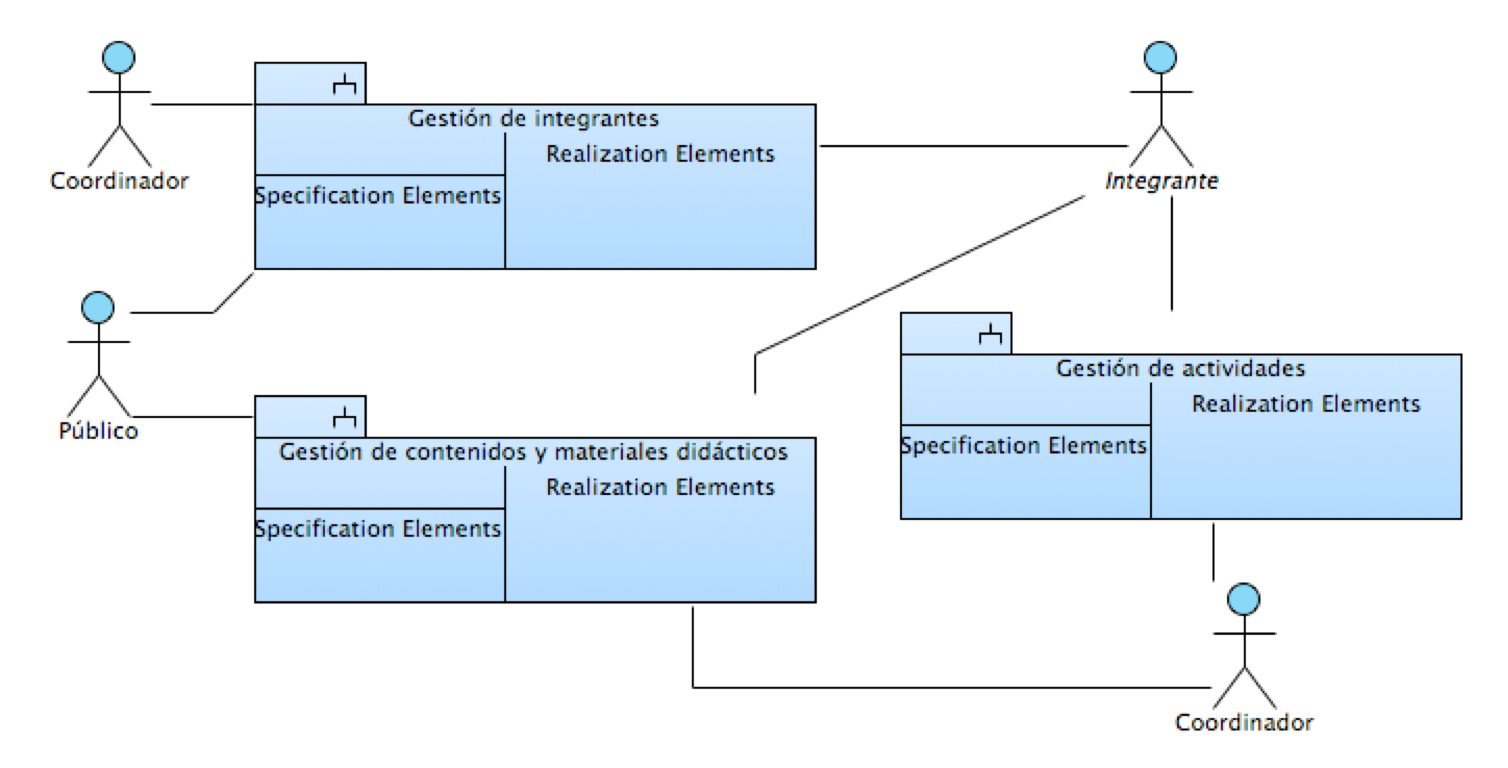
\includegraphics[width=.8\textwidth]{images/casosDeUso}}
		\caption{Diagrama de casos de uso del sistema.}
		\label{fig:casosDeUso}
	\end{center}
\end{figure}

\begin{figure}[htbp]
	\begin{center}
		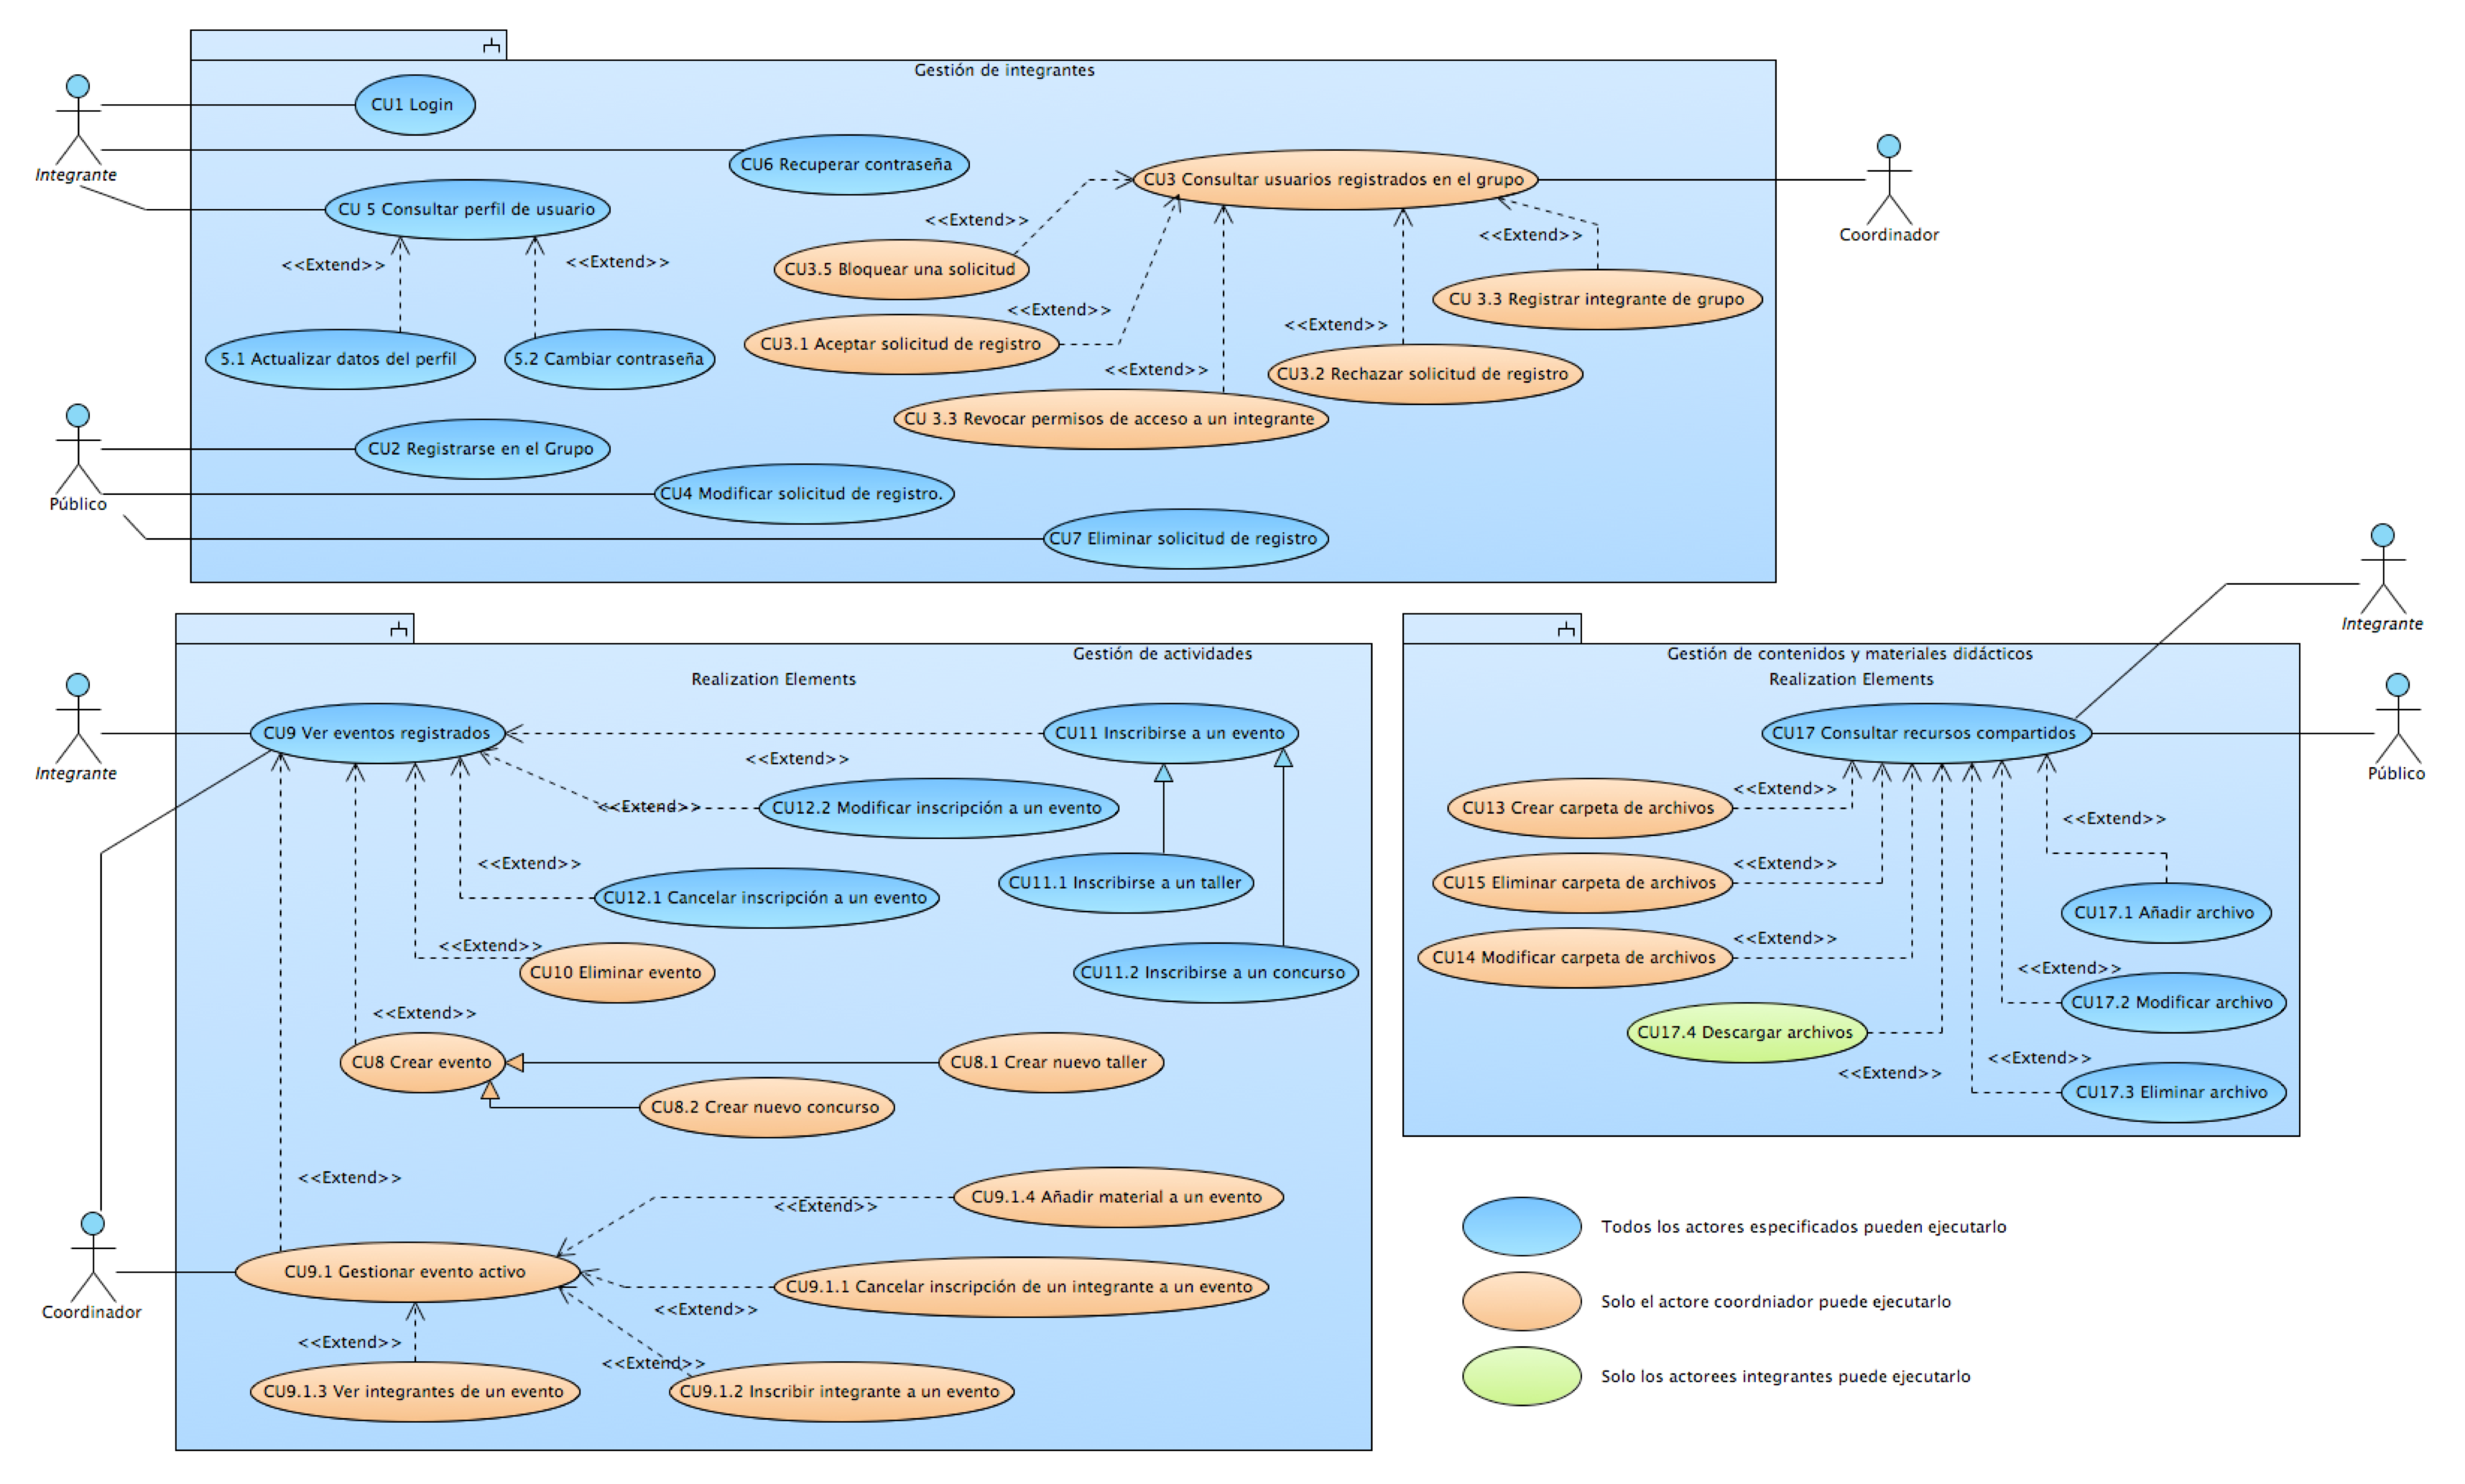
\includegraphics[angle=90, width=.7\textwidth]{images/casosDeUsoDetalle}
		\caption{Diagrama detallado del sistema.}
		\label{fig:casosDeUsoDetalle}
	\end{center}
\end{figure}

%---------------------------------------------------------
\section{Descripción de casos de uso}



A continuación se detallan los casos de uso.

%---------------------------------------------------------
% CASOS DE USO

%-------------------------------------- COMIENZA CU-01
\begin{UseCase}{CU-01}{Iniciar sesión}{
	El usuario del sistema proporciona sus credenciales de acceso para autenticarse e ingresar a los módulos de SICORRE según el rol que tiene asignado.
}
	\UCitem{Versión}{1.0}
	\UCitem{Autor}{Estévez Pérez Alison Beatriz}
	\UCitem{Supervisa}{Pulido Robles Daniel Alfonso}
	\UCitem{Actor}{\hyperlink{Actor.Usuario}{Usuario (Administrador / Especialista)}}
	\UCitem{Propósito}{\begin{Titemize}
		\Titem Controlar el acceso al sistema para proteger la información confidencial de los NNA.
	\end{Titemize}
	}\UCitem{Entradas}{\begin{Titemize}
		\Titem \hyperlink{usuarios.correo}{Correo electrónico}.
		\Titem \hyperlink{usuarios.contrasena}{Contraseña}.
	\end{Titemize}
	}\UCitem{Origen}{\begin{Titemize}
		\Titem Se introducen desde el teclado en la pantalla de inicio de sesión.
	\end{Titemize}
	}\UCitem{Salidas}{\begin{Titemize}
		\Titem Redirección al panel principal correspondiente a su rol.
		\Titem Mensajes de error en caso de credenciales inválidas.
	\end{Titemize}
	}\UCitem{Destino}{\begin{Titemize}
		\Titem Pantalla \IUref{IU-01}{Iniciar sesión}.
	\end{Titemize}
	}\UCitem{Precondiciones}{\begin{Titemize}
		\Titem El usuario debe estar registrado y activo en el sistema.
	\end{Titemize}
	}\UCitem{Postcondiciones}{\begin{Titemize}
		\Titem Se inicia una sesión activa para el usuario en el sistema.
	\end{Titemize}
	}\UCitem{Errores}{\begin{Titemize}
		\Titem {\bf \hypertarget{CU-01.E1}{E1}}: Credenciales incorrectas; el sistema muestra ``Correo o contraseña inválidos'' y regresa al paso \ref{CU-01.ingresaCredenciales}.
	\end{Titemize}
	}\UCitem{Tipo}{
		Caso de uso primario.
	}\UCitem{Observaciones}{
		Ninguna.
	}
\end{UseCase}

\begin{UCtrayectoria}
	\UCpaso[\UCactor] Accede a la URL del sistema.
	\UCpaso Muestra la pantalla \IUref{IU-01}{Iniciar sesión}.
	\UCpaso[\UCactor] \label{CU-01.ingresaCredenciales} Ingresa su correo electrónico y contraseña, y presiona \IUbutton{Ingresar}.
	\UCpaso Valida las credenciales ingresadas. \ErrorRef{CU-01}{E1}{Credenciales incorrectas}
	\UCpaso Verifica el rol del usuario y crea la sesión.
	\UCpaso Redirige al panel principal (Dashboard).
\end{UCtrayectoria}
%-------------------------------------- TERMINA CU-01

%-------------------------------------- COMIENZA CU-02
\begin{UseCase}{CU-02}{Cerrar sesión}{
	El usuario del sistema solicita finalizar su sesión activa para evitar accesos no autorizados a su cuenta y a la información del sistema.
}
	\UCitem{Versión}{1.0}
	\UCitem{Autor}{Estévez Pérez Alison Beatriz}
	\UCitem{Supervisa}{Pulido Robles Daniel Alfonso}
	\UCitem{Actor}{\hyperlink{Actor.Usuario}{Usuario (Administrador / Especialista)}}
	\UCitem{Propósito}{\begin{Titemize}
		\Titem Proteger la cuenta del usuario cerrando el acceso seguro al sistema.
	\end{Titemize}
	}\UCitem{Entradas}{\begin{Titemize}
		\Titem Ninguna (interacción de botón).
	\end{Titemize}
	}\UCitem{Origen}{\begin{Titemize}
		\Titem Selección de la opción en el menú del sistema.
	\end{Titemize}
	}\UCitem{Salidas}{\begin{Titemize}
		\Titem Pantalla de inicio de sesión.
	\end{Titemize}
	}\UCitem{Destino}{\begin{Titemize}
		\Titem Pantalla \IUref{IU-01}{Iniciar sesión}.
	\end{Titemize}
	}\UCitem{Precondiciones}{\begin{Titemize}
		\Titem El usuario debe tener una sesión activa.
	\end{Titemize}
	}\UCitem{Postcondiciones}{\begin{Titemize}
		\Titem La sesión del usuario es destruida en el servidor.
	\end{Titemize}
	}\UCitem{Errores}{\begin{Titemize}
		\Titem Ninguno.
	\end{Titemize}
	}\UCitem{Tipo}{
		Caso de uso primario.
	}\UCitem{Observaciones}{
		Ninguna.
	}
\end{UseCase}

\begin{UCtrayectoria}
	\UCpaso[\UCactor] Selecciona la opción ``Cerrar sesión'' desde el menú principal o perfil.
	\UCpaso Destruye la sesión activa del usuario.
	\UCpaso Redirige a la pantalla \IUref{IU-01}{Iniciar sesión}.
\end{UCtrayectoria}
%-------------------------------------- TERMINA CU-02

%-------------------------------------- COMIENZA CU-03
\begin{UseCase}{CU-03}{Recuperar contraseña}{
	El usuario del sistema ha olvidado su contraseña y solicita restablecerla. El sistema verifica la identidad del usuario mediante su correo electrónico registrado y, si es válido, envía un correo con instrucciones para crear una nueva contraseña.
}
	\UCitem{Versión}{1.0}
	\UCitem{Autor}{Estévez Pérez Alison Beatriz}
	\UCitem{Supervisa}{Pulido Robles Daniel Alfonso}
	\UCitem{Actor}{\hyperlink{Actor.Usuario}{Usuario (Administrador / Especialista)}}
	\UCitem{Propósito}{\begin{Titemize}
		\Titem Permitir al usuario recuperar el acceso al sistema cuando ha olvidado su contraseña.
		\Titem Garantizar que únicamente el propietario legítimo del correo registrado pueda restablecer la contraseña.
	\end{Titemize}
	}\UCitem{Entradas}{\begin{Titemize}
		\Titem \hyperlink{usuarios.correo}{Correo electrónico del usuario}.
	\end{Titemize}
	}\UCitem{Origen}{\begin{Titemize}
		\Titem Se introduce desde el teclado en la pantalla de recuperación de contraseña.
	\end{Titemize}
	}\UCitem{Salidas}{\begin{Titemize}
		\Titem Mensaje de confirmación indicando que se ha enviado el correo de recuperación.
		\Titem Correo electrónico con enlace temporal para restablecer la contraseña.
		\Titem Mensaje de error en caso de que el correo no esté registrado.
	\end{Titemize}
	}\UCitem{Destino}{\begin{Titemize}
		\Titem Se muestra en la pantalla \IUref{IU-03}{Recuperar contraseña}.
		\Titem Se envía al correo electrónico registrado del usuario.
	\end{Titemize}
	}\UCitem{Precondiciones}{\begin{Titemize}
		\Titem El usuario debe tener una cuenta registrada en el sistema con correo electrónico válido.
		\Titem El usuario debe estar en la pantalla de inicio de sesión.
		\Titem La cuenta del usuario debe estar activa en el sistema.
	\end{Titemize}
	}\UCitem{Postcondiciones}{\begin{Titemize}
		\Titem Se genera un token temporal único vinculado al usuario en la base de datos.
		\Titem Se envía un correo electrónico al usuario con el enlace de restablecimiento.
		\Titem La contraseña anterior permanece vigente hasta que el usuario establezca una nueva.
	\end{Titemize}
	}\UCitem{Errores}{\begin{Titemize}
		\Titem {\bf \hypertarget{CU-03.E1}{E1}}: El correo electrónico ingresado no está registrado en el sistema; el sistema muestra el mensaje ``El correo ingresado no está asociado a ninguna cuenta'' y regresa al paso \ref{CU-03.ingresaCorreo}.
		\Titem {\bf \hypertarget{CU-03.E2}{E2}}: La cuenta asociada al correo se encuentra inactiva (revocada); el sistema muestra el mensaje ``El acceso ha sido revocado. Contacte al administrador'' y termina el caso de uso.
		\Titem {\bf \hypertarget{CU-03.E3}{E3}}: El campo de correo electrónico se envía vacío; el sistema muestra el mensaje ``El campo Correo electrónico es requerido'' y regresa al paso \ref{CU-03.ingresaCorreo}.
	\end{Titemize}
	}\UCitem{Tipo}{
		Caso de uso primario.
	}\UCitem{Observaciones}{
		El enlace de recuperación debe tener una vigencia máxima de 24 horas por razones de seguridad. Dado que el sistema maneja datos sensibles de menores, el proceso de recuperación debe registrarse en la bitácora del sistema.
	}
\end{UseCase}

\begin{UCtrayectoria}
	\UCpaso[\UCactor] Solicita recuperar su contraseña seleccionando la opción ``¿Olvidé mi contraseña?'' en la pantalla \IUref{IU-01}{Iniciar sesión}.
	\UCpaso Muestra la pantalla \IUref{IU-03}{Recuperar contraseña} con un campo para ingresar el correo electrónico.
	\UCpaso[\UCactor] \label{CU-03.ingresaCorreo} Ingresa su correo electrónico registrado y presiona el botón \IUbutton{Enviar}.
	\UCpaso Valida que el campo no esté vacío. \ErrorRef{CU-03}{E3}{Campo vacío}
	\UCpaso Busca el correo ingresado en la tabla \hyperlink{usuarios}{usuarios}. \ErrorRef{CU-03}{E1}{Correo no registrado}
	\UCpaso Verifica que la cuenta asociada al correo se encuentre activa. \ErrorRef{CU-03}{E2}{Cuenta inactiva}
	\UCpaso Genera un token temporal de recuperación y lo almacena en el sistema con su fecha de expiración.
	\UCpaso Envía un correo electrónico al usuario con el enlace de recuperación y las instrucciones para restablecer su contraseña.
	\UCpaso Muestra en pantalla el mensaje ``Se ha enviado un correo de recuperación a la dirección indicada. Revise su bandeja de entrada.''
\end{UCtrayectoria}
%-------------------------------------- TERMINA CU-03

%-------------------------------------- COMIENZA CU-04
\begin{UseCase}{CU-04}{Registrar usuario}{
	El administrador del sistema registra un nuevo usuario (especialista o administrador) proporcionando sus datos personales, correo electrónico y asignándole un perfil/rol específico con contraseña temporal.
}
	\UCitem{Versión}{1.0}
	\UCitem{Autor}{Estévez Pérez Alison Beatriz}
	\UCitem{Supervisa}{Pulido Robles Daniel Alfonso}
	\UCitem{Actor}{\hyperlink{Actor.Administrador}{Administrador}}
	\UCitem{Propósito}{\begin{Titemize}
		\Titem Otorgar acceso al sistema al personal autorizado de la institución.
	\end{Titemize}
	}\UCitem{Entradas}{\begin{Titemize}
		\Titem \hyperlink{usuarios.nombre}{Nombre completo}, \hyperlink{usuarios.correo}{Correo electrónico}.
		\Titem \hyperlink{usuarios.rol}{Rol del usuario} (Administrador / Especialista).
	\end{Titemize}
	}\UCitem{Origen}{\begin{Titemize}
		\Titem Pantalla de registro de usuarios.
	\end{Titemize}
	}\UCitem{Salidas}{\begin{Titemize}
		\Titem Mensaje de registro exitoso, envío de correo con contraseña temporal.
	\end{Titemize}
	}\UCitem{Destino}{\begin{Titemize}
		\Titem Base de datos; correo del nuevo usuario.
	\end{Titemize}
	}\UCitem{Precondiciones}{\begin{Titemize}
		\Titem El administrador debe haber iniciado sesión.
	\end{Titemize}
	}\UCitem{Postcondiciones}{\begin{Titemize}
		\Titem Usuario creado y en estado activo.
	\end{Titemize}
	}\UCitem{Errores}{\begin{Titemize}
		\Titem {\bf \hypertarget{CU-04.E1}{E1}}: El correo ingresado ya existe; el sistema muestra ``El correo ya pertenece a otro usuario''.
	\end{Titemize}
	}\UCitem{Tipo}{
		Caso de uso primario.
	}\UCitem{Observaciones}{
		Ninguna.
	}
\end{UseCase}

\begin{UCtrayectoria}
	\UCpaso[\UCactor] Selecciona la opción para registrar un nuevo usuario desde el panel de administración.
	\UCpaso Muestra el formulario \IUref{IU-04}{Registrar usuario}.
	\UCpaso[\UCactor] Ingresa los datos solicitados y presiona \IUbutton{Guardar}.
	\UCpaso Verifica que el correo electrónico no esté en uso. \ErrorRef{CU-04}{E1}{Correo duplicado}
	\UCpaso Registra al usuario y genera una contraseña inicial.
	\UCpaso Muestra el mensaje de éxito.
\end{UCtrayectoria}
%-------------------------------------- TERMINA CU-04

%-------------------------------------- COMIENZA CU-05
\begin{UseCase}{CU-05}{Consultar usuario}{
	El administrador visualiza la lista de usuarios del sistema y revisa el detalle de un usuario específico, verificando su información, rol y estado.
}
	\UCitem{Versión}{1.0}
	\UCitem{Autor}{Estévez Pérez Alison Beatriz}
	\UCitem{Supervisa}{Pulido Robles Daniel Alfonso}
	\UCitem{Actor}{\hyperlink{Actor.Administrador}{Administrador}}
	\UCitem{Propósito}{\begin{Titemize}
		\Titem Consultar rápidamente los datos y actividad de los empleados con acceso.
	\end{Titemize}
	}\UCitem{Entradas}{\begin{Titemize}
		\Titem Criterio de búsqueda (nombre o correo).
	\end{Titemize}
	}\UCitem{Origen}{\begin{Titemize}
		\Titem Pantalla general de usuarios.
	\end{Titemize}
	}\UCitem{Salidas}{\begin{Titemize}
		\Titem Datos del usuario seleccionado.
	\end{Titemize}
	}\UCitem{Destino}{\begin{Titemize}
		\Titem Pantalla \IUref{IU-05}{Consultar usuario}.
	\end{Titemize}
	}\UCitem{Precondiciones}{\begin{Titemize}
		\Titem El administrador ha iniciado sesión.
	\end{Titemize}
	}\UCitem{Postcondiciones}{\begin{Titemize}
		\Titem Ninguna (sólo lectura).
	\end{Titemize}
	}\UCitem{Errores}{\begin{Titemize}
		\Titem Ninguno.
	\end{Titemize}
	}\UCitem{Tipo}{
		Caso de uso secundario.
	}\UCitem{Observaciones}{
		Ninguna.
	}
\end{UseCase}

\begin{UCtrayectoria}
	\UCpaso[\UCactor] Ingresa al módulo de gestión de usuarios.
	\UCpaso Muestra el listado de usuarios registrados en el sistema.
	\UCpaso[\UCactor] Opcionalmente ingresa un texto para filtrar y selecciona al usuario.
	\UCpaso Despliega los detalles de perfil del usuario seleccionado.
\end{UCtrayectoria}
%-------------------------------------- TERMINA CU-05

%-------------------------------------- COMIENZA CU-06
\begin{UseCase}{CU-06}{Modificar usuario}{
	El administrador del sistema actualiza los datos personales, de contacto o el nivel de rol de un usuario previamente registrado.
}
	\UCitem{Versión}{1.0}
	\UCitem{Autor}{Estévez Pérez Alison Beatriz}
	\UCitem{Supervisa}{Pulido Robles Daniel Alfonso}
	\UCitem{Actor}{\hyperlink{Actor.Administrador}{Administrador}}
	\UCitem{Propósito}{\begin{Titemize}
		\Titem Mantener la vigencia de la información de cuenta de los trabajadores en el sistema.
	\end{Titemize}
	}\UCitem{Entradas}{\begin{Titemize}
		\Titem Datos del usuario (modificables como nombre y rol).
	\end{Titemize}
	}\UCitem{Origen}{\begin{Titemize}
		\Titem Pantalla de edición de usuario.
	\end{Titemize}
	}\UCitem{Salidas}{\begin{Titemize}
		\Titem Confirmación de actualización.
	\end{Titemize}
	}\UCitem{Destino}{\begin{Titemize}
		\Titem Base de datos.
	\end{Titemize}
	}\UCitem{Precondiciones}{\begin{Titemize}
		\Titem El administrador ha iniciado sesión y ha localizado al usuario.
	\end{Titemize}
	}\UCitem{Postcondiciones}{\begin{Titemize}
		\Titem Datos del usuario modificados en base de datos.
	\end{Titemize}
	}\UCitem{Errores}{\begin{Titemize}
		\Titem {\bf \hypertarget{CU-06.E1}{E1}}: Campos vacíos obligatorios; sistema pide rellenarlos.
	\end{Titemize}
	}\UCitem{Tipo}{
		Caso de uso primario.
	}\UCitem{Observaciones}{
		Si se modifica el correo, se debe confirmar que no pertenezca a otra cuenta.
	}
\end{UseCase}

\begin{UCtrayectoria}
	\UCpaso[\UCactor] Selecciona la opción de edición en el perfil del usuario.
	\UCpaso Muestra la pantalla \IUref{IU-06}{Modificar usuario} con los datos actuales prellenados.
	\UCpaso[\UCactor] Actualiza los datos y presiona el botón \IUbutton{Actualizar}.
	\UCpaso Valida los campos ingresados. \ErrorRef{CU-06}{E1}{Campos inválidos}
	\UCpaso Persiste la nueva información en la tabla de usuarios.
	\UCpaso Indica que los cambios fueron guardados exitosamente.
\end{UCtrayectoria}
%-------------------------------------- TERMINA CU-06

%-------------------------------------- COMIENZA CU-07
\begin{UseCase}{CU-07}{Revocar acceso a usuario}{
	El administrador del sistema inhabilita permanentemente o temporalmente el acceso de un usuario específico cambiándolo de estatus activo a inactivo/revocado.
}
	\UCitem{Versión}{1.0}
	\UCitem{Autor}{Estévez Pérez Alison Beatriz}
	\UCitem{Supervisa}{Pulido Robles Daniel Alfonso}
	\UCitem{Actor}{\hyperlink{Actor.Administrador}{Administrador}}
	\UCitem{Propósito}{\begin{Titemize}
		\Titem Controlar los accesos de exempleados o cuentas comprometidas.
	\end{Titemize}
	}\UCitem{Entradas}{\begin{Titemize}
		\Titem Identificador del usuario.
	\end{Titemize}
	}\UCitem{Origen}{\begin{Titemize}
		\Titem Botón en la interfaz de gestión.
	\end{Titemize}
	}\UCitem{Salidas}{\begin{Titemize}
		\Titem Mensaje confirmando la inhabilitación.
	\end{Titemize}
	}\UCitem{Destino}{\begin{Titemize}
		\Titem Base de datos (cambio de estado).
	\end{Titemize}
	}\UCitem{Precondiciones}{\begin{Titemize}
		\Titem El usuario a inhabilitar debe estar actualmente activo.
	\end{Titemize}
	}\UCitem{Postcondiciones}{\begin{Titemize}
		\Titem El usuario no podrá iniciar sesión en el futuro, pero su historial se conserva.
	\end{Titemize}
	}\UCitem{Errores}{\begin{Titemize}
		\Titem Ninguno.
	\end{Titemize}
	}\UCitem{Tipo}{
		Caso de uso primario.
	}\UCitem{Observaciones}{
		Alternativa preferida antes de eliminar el registro.
	}
\end{UseCase}

\begin{UCtrayectoria}
	\UCpaso[\UCactor] Selecciona la opción ``Desactivar'' o ``Revocar'' sobre un usuario del listado.
	\UCpaso Pide confirmación sobre la inhabilitación.
	\UCpaso[\UCactor] Confirma la decisión.
	\UCpaso Cambia el estatus vinculante del usuario en la base de datos a `inactivo`.
	\UCpaso Notifica el éxito de la revocación.
\end{UCtrayectoria}
%-------------------------------------- TERMINA CU-07

%-------------------------------------- COMIENZA CU-08
\begin{UseCase}{CU-08}{Eliminar usuario}{
	El administrador efectúa la eliminación definitiva de un usuario del sistema sólo si éste no cuenta con integraciones activas como expedientes relacionados o asignaciones en equipos multidisciplinarios.
}
	\UCitem{Versión}{1.0}
	\UCitem{Autor}{Estévez Pérez Alison Beatriz}
	\UCitem{Supervisa}{Pulido Robles Daniel Alfonso}
	\UCitem{Actor}{\hyperlink{Actor.Administrador}{Administrador}}
	\UCitem{Propósito}{\begin{Titemize}
		\Titem Eliminar registros errados o cuentas que no han sido utilizadas y no cuentan con historial.
	\end{Titemize}
	}\UCitem{Entradas}{\begin{Titemize}
		\Titem Identificador del usuario.
	\end{Titemize}
	}\UCitem{Origen}{\begin{Titemize}
		\Titem Acción desde la interfaz de consulta.
	\end{Titemize}
	}\UCitem{Salidas}{\begin{Titemize}
		\Titem Mensaje de exclusión exitosa o alerta si la eliminación no es posible.
	\end{Titemize}
	}\UCitem{Destino}{\begin{Titemize}
		\Titem Base de datos.
	\end{Titemize}
	}\UCitem{Precondiciones}{\begin{Titemize}
		\Titem Usuario seleccionado no debe estar inmerso en alguna bitácora de casos críticos o como especialista único de algún NNA.
	\end{Titemize}
	}\UCitem{Postcondiciones}{\begin{Titemize}
		\Titem El registro desaparece lógicamente de la plataforma.
	\end{Titemize}
	}\UCitem{Errores}{\begin{Titemize}
		\Titem {\bf \hypertarget{CU-08.E1}{E1}}: El usuario tiene expedientes asociados; el sistema bloquea el borrado e indica que primero se le debe retirar la carga de trabajo o en su defecto, revocar el acceso en lugar de eliminar.
	\end{Titemize}
	}\UCitem{Tipo}{
		Caso de uso primario.
	}\UCitem{Observaciones}{
		Normalmente se prioriza revocar acceso; la eliminación sólo aplica a captura equivocada.
	}
\end{UseCase}

\begin{UCtrayectoria}
	\UCpaso[\UCactor] En el panel administrativo, elige ``Eliminar usuario''.
	\UCpaso Muestra ventana de comprobación informando las implicaciones.
	\UCpaso[\UCactor] Confirma su voluntad de eliminar.
	\UCpaso Comprueba dependencias de integridad referencial vinculadas al usuario. \ErrorRef{CU-08}{E1}{Usuario con expedientes asignados}
	\UCpaso Procede al borrado de la cuenta.
	\UCpaso Muestra la notificación de conclusión de la tarea.
\end{UCtrayectoria}
%-------------------------------------- TERMINA CU-08

%-------------------------------------- COMIENZA CU-09
\begin{UseCase}{CU-09}{Registrar equipo multidisciplinario}{
	El administrador del sistema accede al módulo de equipos multidisciplinarios y registra un nuevo equipo proporcionando su nombre. El sistema valida que el nombre no esté duplicado y almacena el nuevo equipo como activo en la base de datos.
}
	\UCitem{Versión}{1.0}
	\UCitem{Autor}{Estévez Pérez Alison Beatriz}
	\UCitem{Supervisa}{Pulido Robles Daniel Alfonso}
	\UCitem{Actor}{\hyperlink{Actor.Administrador}{Administrador}}
	\UCitem{Propósito}{\begin{Titemize}
		\Titem Dar de alta un nuevo equipo multidisciplinario en el sistema para la atención de NNA.
		\Titem Permitir la posterior asignación de integrantes y NNA al equipo creado.
	\end{Titemize}
	}\UCitem{Entradas}{\begin{Titemize}
		\Titem \hyperlink{equipos_multidisciplinarios.nombre_equipo}{Nombre del equipo}.
	\end{Titemize}
	}\UCitem{Origen}{\begin{Titemize}
		\Titem Se introduce desde el teclado en la pantalla de registro de equipo.
	\end{Titemize}
	}\UCitem{Salidas}{\begin{Titemize}
		\Titem Mensaje de confirmación de registro exitoso.
		\Titem El nuevo equipo aparece en el listado de equipos activos.
		\Titem Mensajes de error en caso de datos inválidos o duplicados.
	\end{Titemize}
	}\UCitem{Destino}{\begin{Titemize}
		\Titem Se muestra en la pantalla \IUref{IU-09}{Registrar equipo multidisciplinario}.
		\Titem Se almacena en la tabla \hyperlink{equipos_multidisciplinarios}{equipos\_multidisciplinarios} de la base de datos.
	\end{Titemize}
	}\UCitem{Precondiciones}{\begin{Titemize}
		\Titem El administrador debe haber iniciado sesión en el sistema (\UCref{CU-01}{Iniciar sesión}).
		\Titem El actor debe tener el rol de Administrador en el sistema.
	\end{Titemize}
	}\UCitem{Postcondiciones}{\begin{Titemize}
		\Titem Se registra un nuevo equipo en la tabla \hyperlink{equipos_multidisciplinarios}{equipos\_multidisciplinarios} con estatus activo.
		\Titem Se registra automáticamente la fecha de creación del equipo.
		\Titem El equipo queda disponible para la asignación de integrantes y NNA.
	\end{Titemize}
	}\UCitem{Errores}{\begin{Titemize}
		\Titem {\bf \hypertarget{CU-09.E1}{E1}}: El campo de nombre del equipo se envía vacío; el sistema muestra el mensaje ``El campo Nombre del equipo es requerido'' y regresa al paso \ref{CU-09.ingresaDatos}.
		\Titem {\bf \hypertarget{CU-09.E2}{E2}}: Ya existe un equipo con el mismo nombre en el sistema; el sistema muestra el mensaje ``El nombre de equipo ingresado ya existe en el sistema'' y regresa al paso \ref{CU-09.ingresaDatos}.
	\end{Titemize}
	}\UCitem{Tipo}{
		Caso de uso primario.
	}\UCitem{Observaciones}{
		Ninguna.
	}
\end{UseCase}

\begin{UCtrayectoria}
	\UCpaso[\UCactor] Solicita registrar un nuevo equipo multidisciplinario seleccionando la opción correspondiente en el menú del sistema.
	\UCpaso Muestra la pantalla \IUref{IU-09}{Registrar equipo multidisciplinario} con el formulario de registro.
	\UCpaso[\UCactor] \label{CU-09.ingresaDatos} Ingresa el nombre del equipo y presiona el botón \IUbutton{Guardar}.
	\UCpaso Valida que el campo nombre no esté vacío. \ErrorRef{CU-09}{E1}{Campo vacío}
	\UCpaso Verifica que no exista otro equipo con el mismo nombre en la tabla \hyperlink{equipos_multidisciplinarios}{equipos\_multidisciplinarios}. \ErrorRef{CU-09}{E2}{Nombre duplicado}
	\UCpaso Registra el nuevo equipo en la base de datos con estatus activo y la fecha de creación actual.
	\UCpaso Muestra el mensaje de confirmación ``El equipo multidisciplinario ha sido registrado exitosamente'' y actualiza el listado de equipos.
\end{UCtrayectoria}
%-------------------------------------- TERMINA CU-09
%-------------------------------------- COMIENZA CU-10
\begin{UseCase}{CU-10}{Consultar equipo multidisciplinario}{
	El usuario del sistema accede al módulo de equipos multidisciplinarios y consulta la información de un equipo existente, incluyendo sus integrantes y los NNA asignados a dicho equipo.
}
	\UCitem{Versión}{1.0}
	\UCitem{Autor}{Estévez Pérez Alison Beatriz}
	\UCitem{Supervisa}{Pulido Robles Daniel Alfonso}
	\UCitem{Actor}{\hyperlink{Actor.Usuario}{Usuario (Administrador / Especialista)}}
	\UCitem{Propósito}{\begin{Titemize}
		\Titem Permitir al usuario visualizar la información completa de un equipo multidisciplinario.
		\Titem Facilitar la revisión de los integrantes y los NNA bajo responsabilidad del equipo.
	\end{Titemize}
	}\UCitem{Entradas}{\begin{Titemize}
		\Titem \hyperlink{equipos_multidisciplinarios.nombre_equipo}{Nombre o identificador del equipo} (para búsqueda).
	\end{Titemize}
	}\UCitem{Origen}{\begin{Titemize}
		\Titem Se selecciona desde el listado de equipos o se introduce desde el teclado en el campo de búsqueda.
	\end{Titemize}
	}\UCitem{Salidas}{\begin{Titemize}
		\Titem \hyperlink{equipos_multidisciplinarios.nombre_equipo}{Nombre del equipo}.
		\Titem \hyperlink{equipos_multidisciplinarios.activo}{Estatus del equipo} (Activo / Inactivo).
		\Titem \hyperlink{equipos_multidisciplinarios.fecha_creacion}{Fecha de creación}.
		\Titem Listado de integrantes del equipo con su rol y fecha de ingreso.
		\Titem Listado de NNA asignados al equipo.
		\Titem Mensaje de error si el equipo no existe.
	\end{Titemize}
	}\UCitem{Destino}{\begin{Titemize}
		\Titem Se muestra en la pantalla \IUref{IU-10}{Consultar equipo multidisciplinario}.
	\end{Titemize}
	}\UCitem{Precondiciones}{\begin{Titemize}
		\Titem El usuario debe haber iniciado sesión en el sistema (\UCref{CU-01}{Iniciar sesión}).
		\Titem Debe existir al menos un equipo registrado en el sistema.
	\end{Titemize}
	}\UCitem{Postcondiciones}{\begin{Titemize}
		\Titem No se realizan modificaciones en la base de datos (operación de sólo lectura).
	\end{Titemize}
	}\UCitem{Errores}{\begin{Titemize}
		\Titem {\bf \hypertarget{CU-10.E1}{E1}}: No se encuentran equipos registrados en el sistema; se muestra el mensaje ``No existen equipos multidisciplinarios registrados'' y el listado aparece vacío.
		\Titem {\bf \hypertarget{CU-10.E2}{E2}}: El término de búsqueda ingresado no coincide con ningún equipo; el sistema muestra el mensaje ``No se encontraron resultados para la búsqueda realizada'' y regresa al paso \ref{CU-10.selecciona}.
	\end{Titemize}
	}\UCitem{Tipo}{
		Caso de uso primario.
	}\UCitem{Observaciones}{
		Ninguna.
	}
\end{UseCase}

\begin{UCtrayectoria}
	\UCpaso[\UCactor] Ingresa al módulo de equipos multidisciplinarios desde el menú principal del sistema.
	\UCpaso Muestra la pantalla \IUref{IU-10}{Consultar equipo multidisciplinario} con el listado de todos los equipos registrados. \ErrorRef{CU-10}{E1}{Sin equipos}
	\UCpaso[\UCactor] \label{CU-10.selecciona} Selecciona el equipo que desea consultar del listado, o ingresa un criterio de búsqueda y presiona el botón \IUbutton{Buscar}. \ErrorRef{CU-10}{E2}{Sin resultados}
	\UCpaso Recupera de la base de datos la información del equipo seleccionado, incluyendo sus integrantes actuales de la tabla \hyperlink{integrantes_equipo}{integrantes\_equipo} y los NNA asignados de la tabla \hyperlink{nna}{nna}.
	\UCpaso Muestra la información completa del equipo en la pantalla \IUref{IU-10}{Consultar equipo multidisciplinario}.
\end{UCtrayectoria}
%-------------------------------------- TERMINA CU-10
%-------------------------------------- COMIENZA CU-11
\begin{UseCase}{CU-11}{Modificar equipo multidisciplinario}{
	El administrador del sistema accede a la información de un equipo multidisciplinario existente y realiza modificaciones sobre sus datos o sus integrantes. El sistema valida la información actualizada y persiste los cambios en la base de datos.
}
	\UCitem{Versión}{1.0}
	\UCitem{Autor}{Estévez Pérez Alison Beatriz}
	\UCitem{Supervisa}{Pulido Robles Daniel Alfonso}
	\UCitem{Actor}{\hyperlink{Actor.Administrador}{Administrador}}
	\UCitem{Propósito}{\begin{Titemize}
		\Titem Mantener actualizada la información de los equipos multidisciplinarios registrados en el sistema.
		\Titem Permitir la incorporación o salida de integrantes del equipo registrando el motivo del cambio.
	\end{Titemize}
	}\UCitem{Entradas}{\begin{Titemize}
		\Titem \hyperlink{equipos_multidisciplinarios.nombre_equipo}{Nombre del equipo} (modificable).
		\Titem \hyperlink{equipos_multidisciplinarios.activo}{Estatus del equipo} (Activo / Inactivo).
		\Titem \hyperlink{integrantes_equipo.usuario_id}{Integrante a agregar o dar de baja}.
		\Titem \hyperlink{integrantes_equipo.motivo_cambio}{Motivo del cambio de integrante} (en caso de baja).
		\Titem \hyperlink{integrantes_equipo.fecha_salida}{Fecha de salida del integrante} (en caso de baja).
	\end{Titemize}
	}\UCitem{Origen}{\begin{Titemize}
		\Titem Se introducen o seleccionan desde la pantalla de modificación del equipo.
	\end{Titemize}
	}\UCitem{Salidas}{\begin{Titemize}
		\Titem Mensaje de confirmación de actualización exitosa.
		\Titem Datos actualizados del equipo reflejados en el listado.
		\Titem Mensajes de error en caso de datos inválidos.
	\end{Titemize}
	}\UCitem{Destino}{\begin{Titemize}
		\Titem Se muestra en la pantalla \IUref{IU-11}{Modificar equipo multidisciplinario}.
		\Titem Los cambios se persisten en las tablas \hyperlink{equipos_multidisciplinarios}{equipos\_multidisciplinarios} e \hyperlink{integrantes_equipo}{integrantes\_equipo}.
	\end{Titemize}
	}\UCitem{Precondiciones}{\begin{Titemize}
		\Titem El administrador debe haber iniciado sesión en el sistema (\UCref{CU-01}{Iniciar sesión}).
		\Titem Debe existir el equipo que se desea modificar.
		\Titem El administrador debe haber consultado previamente el equipo (\UCref{CU-10}{Consultar equipo multidisciplinario}).
	\end{Titemize}
	}\UCitem{Postcondiciones}{\begin{Titemize}
		\Titem Se actualizan los datos del equipo en la tabla \hyperlink{equipos_multidisciplinarios}{equipos\_multidisciplinarios}.
		\Titem En caso de baja de un integrante, se registra la fecha de salida y motivo en \hyperlink{integrantes_equipo}{integrantes\_equipo} con estatus ``Inactivo''.
		\Titem En caso de incorporación de un integrante, se crea un nuevo registro en \hyperlink{integrantes_equipo}{integrantes\_equipo} con la fecha de ingreso actual.
	\end{Titemize}
	}\UCitem{Errores}{\begin{Titemize}
		\Titem {\bf \hypertarget{CU-11.E1}{E1}}: El campo nombre del equipo se deja vacío; el sistema muestra el mensaje ``El campo Nombre del equipo es requerido'' y regresa al paso \ref{CU-11.modificaDatos}.
		\Titem {\bf \hypertarget{CU-11.E2}{E2}}: El nombre modificado ya existe en otro equipo registrado; el sistema muestra el mensaje ``El nombre de equipo ingresado ya existe en el sistema'' y regresa al paso \ref{CU-11.modificaDatos}.
		\Titem {\bf \hypertarget{CU-11.E3}{E3}}: Se intenta dar de baja a un integrante sin especificar el motivo; el sistema muestra el mensaje ``El campo Motivo del cambio es requerido'' y regresa al paso \ref{CU-11.modificaDatos}.
	\end{Titemize}
	}\UCitem{Tipo}{
		Caso de uso primario.
	}\UCitem{Observaciones}{
		El historial de cambios de integrantes debe conservarse para fines de auditoría y no debe eliminarse de la base de datos.
	}
\end{UseCase}

\begin{UCtrayectoria}
	\UCpaso[\UCactor] Selecciona la opción ``Modificar'' sobre el equipo deseado en la pantalla \IUref{IU-10}{Consultar equipo multidisciplinario}.
	\UCpaso Muestra la pantalla \IUref{IU-11}{Modificar equipo multidisciplinario} con los datos actuales del equipo precargados.
	\UCpaso[\UCactor] \label{CU-11.modificaDatos} Realiza los cambios deseados sobre el nombre, estatus o integrantes del equipo y presiona el botón \IUbutton{Guardar cambios}.
	\UCpaso Valida que el campo nombre no esté vacío. \ErrorRef{CU-11}{E1}{Campo vacío}
	\UCpaso Verifica que el nuevo nombre no esté en uso por otro equipo. \ErrorRef{CU-11}{E2}{Nombre duplicado}
	\UCpaso En caso de cambio de integrantes, valida que se haya especificado el motivo de baja. \ErrorRef{CU-11}{E3}{Motivo requerido}
	\UCpaso Persiste los cambios en las tablas correspondientes de la base de datos.
	\UCpaso Muestra el mensaje ``El equipo multidisciplinario ha sido actualizado exitosamente'' y regresa al listado de equipos.
\end{UCtrayectoria}
%-------------------------------------- TERMINA CU-11
%-------------------------------------- COMIENZA CU-12
\begin{UseCase}{CU-12}{Asignar NNA a equipo multidisciplinario}{
	El administrador del sistema selecciona un NNA registrado y lo asigna a un equipo multidisciplinario activo. El sistema valida que el NNA no esté ya asignado a otro equipo y actualiza el registro correspondiente en la base de datos.
}
	\UCitem{Versión}{1.0}
	\UCitem{Autor}{Estévez Pérez Alison Beatriz}
	\UCitem{Supervisa}{Pulido Robles Daniel Alfonso}
	\UCitem{Actor}{\hyperlink{Actor.Administrador}{Administrador}}
	\UCitem{Propósito}{\begin{Titemize}
		\Titem Vincular a un NNA con el equipo multidisciplinario responsable de dar seguimiento a su caso.
		\Titem Garantizar que cada NNA tenga un equipo responsable claramente definido en el sistema.
	\end{Titemize}
	}\UCitem{Entradas}{\begin{Titemize}
		\Titem \hyperlink{nna.id}{Identificador del NNA} a asignar.
		\Titem \hyperlink{equipos_multidisciplinarios.id}{Equipo multidisciplinario} al que se asignará.
	\end{Titemize}
	}\UCitem{Origen}{\begin{Titemize}
		\Titem Se seleccionan desde listas desplegables en la pantalla de asignación.
	\end{Titemize}
	}\UCitem{Salidas}{\begin{Titemize}
		\Titem Mensaje de confirmación de asignación exitosa.
		\Titem El NNA aparece en el listado de NNA del equipo asignado.
		\Titem Mensajes de error en caso de datos inválidos o asignación previa.
	\end{Titemize}
	}\UCitem{Destino}{\begin{Titemize}
		\Titem Se muestra en la pantalla \IUref{IU-12}{Asignar NNA a equipo multidisciplinario}.
		\Titem Se actualiza el campo \hyperlink{nna.equipo_asignado_id}{equipo\_asignado\_id} en la tabla \hyperlink{nna}{nna}.
	\end{Titemize}
	}\UCitem{Precondiciones}{\begin{Titemize}
		\Titem El administrador debe haber iniciado sesión en el sistema (\UCref{CU-01}{Iniciar sesión}).
		\Titem Debe existir al menos un NNA registrado en el sistema (\UCref{CU-13}{Registrar NNA}).
		\Titem Debe existir al menos un equipo multidisciplinario activo (\UCref{CU-09}{Registrar equipo multidisciplinario}).
	\end{Titemize}
	}\UCitem{Postcondiciones}{\begin{Titemize}
		\Titem Se actualiza el campo \hyperlink{nna.equipo_asignado_id}{equipo\_asignado\_id} del NNA seleccionado en la tabla \hyperlink{nna}{nna}.
		\Titem El equipo asignado puede visualizar al NNA en su listado de casos a atender.
	\end{Titemize}
	}\UCitem{Errores}{\begin{Titemize}
		\Titem {\bf \hypertarget{CU-12.E1}{E1}}: No se selecciona un NNA; el sistema muestra el mensaje ``Debe seleccionar un NNA para realizar la asignación'' y regresa al paso \ref{CU-12.selecciona}.
		\Titem {\bf \hypertarget{CU-12.E2}{E2}}: No se selecciona un equipo; el sistema muestra el mensaje ``Debe seleccionar un equipo multidisciplinario'' y regresa al paso \ref{CU-12.selecciona}.
		\Titem {\bf \hypertarget{CU-12.E3}{E3}}: El NNA ya se encuentra asignado al mismo equipo seleccionado; el sistema muestra el mensaje ``El NNA ya se encuentra asignado a este equipo'' y regresa al paso \ref{CU-12.selecciona}.
	\end{Titemize}
	}\UCitem{Tipo}{
		Caso de uso primario.
	}\UCitem{Observaciones}{
		Si el NNA ya tenía un equipo asignado previamente, la nueva asignación reemplaza a la anterior. Se recomienda notificar al administrador de este cambio.
	}
\end{UseCase}

\begin{UCtrayectoria}
	\UCpaso[\UCactor] Accede al módulo de asignación de NNA desde el panel de administración.
	\UCpaso Muestra la pantalla \IUref{IU-12}{Asignar NNA a equipo multidisciplinario} con una lista de NNA disponibles y una lista de equipos activos.
	\UCpaso[\UCactor] \label{CU-12.selecciona} Selecciona el NNA y el equipo multidisciplinario al que desea asignarlo, y presiona el botón \IUbutton{Asignar}. \ErrorRef{CU-12}{E1}{NNA no seleccionado} \ErrorRef{CU-12}{E2}{Equipo no seleccionado}
	\UCpaso Verifica que el NNA no esté ya asignado al mismo equipo seleccionado. \ErrorRef{CU-12}{E3}{Asignación duplicada}
	\UCpaso Actualiza el campo \hyperlink{nna.equipo_asignado_id}{equipo\_asignado\_id} del NNA en la tabla \hyperlink{nna}{nna}.
	\UCpaso Muestra el mensaje ``El NNA ha sido asignado exitosamente al equipo multidisciplinario seleccionado.''
\end{UCtrayectoria}
%-------------------------------------- TERMINA CU-12
%-------------------------------------- COMIENZA CU-13
\begin{UseCase}{CU-13}{Registrar NNA}{
	El especialista autorizado accede al módulo del NNA y captura la información completa del niño, niña o adolescente (NNA) incluyendo sus datos personales, domicilio, estatus escolar, condición migratoria e información de salud. El sistema valida los datos, detecta posibles duplicados y registra al NNA en la base de datos.
}
	\UCitem{Versión}{1.0}
	\UCitem{Autor}{Estévez Pérez Alison Beatriz}
	\UCitem{Supervisa}{Pulido Robles Daniel Alfonso}
	\UCitem{Actor}{\hyperlink{Actor.Especialista}{Especialista (Trabajador/a Social / Psicólogo/a / Abogado/a)}}
	\UCitem{Propósito}{\begin{Titemize}
		\Titem Crear el registro digital del NNA en el sistema SICORRE para dar inicio a su proceso de atención.
		\Titem Evitar la duplicidad de registros mediante la validación de CURP.
		\Titem Centralizar la información del NNA como punto de partida para la apertura de expedientes.
	\end{Titemize}
	}\UCitem{Entradas}{\begin{Titemize}
		\Titem \hyperlink{nna.nombre}{Nombre(s) del NNA}.
		\Titem \hyperlink{nna.primer_apellido}{Primer apellido del NNA}.
		\Titem \hyperlink{nna.segundo_apellido}{Segundo apellido del NNA}.
		\Titem \hyperlink{nna.fecha_nacimiento}{Fecha de nacimiento}.
		\Titem \hyperlink{nna.sexo}{Sexo}.
		\Titem \hyperlink{nna.curp}{CURP} (opcional si no cuenta con él).
		\Titem \hyperlink{nna.nacionalidad}{Nacionalidad}.
		\Titem \hyperlink{nna.es_migrante}{Indicador de condición migrante}.
		\Titem \hyperlink{nna.estatus_escolar_id}{Estatus escolar} (selección del catálogo \hyperlink{cat_estatus_escolar}{cat\_estatus\_escolar}).
		\Titem \hyperlink{direcciones_nna.calle}{Calle}, \hyperlink{direcciones_nna.num_exterior}{número exterior}, \hyperlink{direcciones_nna.num_interior}{número interior}.
		\Titem \hyperlink{direcciones_nna.colonia_id}{Colonia} (del catálogo SEPOMEX).
		\Titem \hyperlink{direcciones_nna.pueblo_comunidad}{Pueblo o comunidad} (en caso de aplicar).
		\Titem \hyperlink{direcciones_nna.vivienda_nna_id}{Tipo de vivienda} (del catálogo \hyperlink{cat_vivienda_nna}{cat\_vivienda\_nna}).
		\Titem \hyperlink{nna.tutor_id}{Tutor del NNA} (referencia al tutor ya registrado).
	\end{Titemize}
	}\UCitem{Origen}{\begin{Titemize}
		\Titem Se introducen desde el teclado o se seleccionan de listas desplegables en la pantalla de registro de NNA.
	\end{Titemize}
	}\UCitem{Salidas}{\begin{Titemize}
		\Titem Mensaje de confirmación de registro exitoso.
		\Titem Número de identificador asignado al NNA en el sistema.
		\Titem Mensajes de error en caso de datos inválidos o duplicados.
	\end{Titemize}
	}\UCitem{Destino}{\begin{Titemize}
		\Titem Se muestra en la pantalla \IUref{IU-13}{Registrar NNA}.
		\Titem Se almacena en las tablas \hyperlink{nna}{nna} y \hyperlink{direcciones_nna}{direcciones\_nna} de la base de datos.
	\end{Titemize}
	}\UCitem{Precondiciones}{\begin{Titemize}
		\Titem El especialista debe haber iniciado sesión en el sistema (\UCref{CU-01}{Iniciar sesión}).
		\Titem El tutor del NNA debe estar registrado previamente en el sistema (\UCref{CU-18}{Registrar tutor del NNA}).
	\end{Titemize}
	}\UCitem{Postcondiciones}{\begin{Titemize}
		\Titem Se crea un nuevo registro en la tabla \hyperlink{nna}{nna} con estatus activo.
		\Titem Se crea el registro de dirección correspondiente en \hyperlink{direcciones_nna}{direcciones\_nna}.
		\Titem Se registra el usuario que realizó el registro en el campo \hyperlink{nna.creado_por}{creado\_por}.
		\Titem El NNA queda disponible para la apertura de expediente y asignación a equipo.
	\end{Titemize}
	}\UCitem{Errores}{\begin{Titemize}
		\Titem {\bf \hypertarget{CU-13.E1}{E1}}: Algún campo obligatorio (nombre, apellidos, fecha de nacimiento) se envía vacío; el sistema muestra el mensaje ``El campo [Nombre\_Campo] es requerido'' y regresa al paso \ref{CU-13.ingresaDatos}.
		\Titem {\bf \hypertarget{CU-13.E2}{E2}}: La CURP ingresada ya existe en el sistema; el sistema muestra el mensaje ``La CURP ingresada ya existe en el sistema. Verifique si el NNA ya fue registrado'' y regresa al paso \ref{CU-13.ingresaDatos}.
		\Titem {\bf \hypertarget{CU-13.E3}{E3}}: La fecha de nacimiento es posterior a la fecha actual; el sistema muestra el mensaje ``La fecha de nacimiento no puede ser mayor a la fecha actual'' y regresa al paso \ref{CU-13.ingresaDatos}.
		\Titem {\bf \hypertarget{CU-13.E4}{E4}}: La CURP no tiene el formato válido de 18 caracteres; el sistema muestra el mensaje ``La CURP debe tener 18 caracteres'' y regresa al paso \ref{CU-13.ingresaDatos}.
	\end{Titemize}
	}\UCitem{Tipo}{
		Caso de uso primario.
	}\UCitem{Observaciones}{
		La información del NNA es de carácter sensible y está protegida por la LGDNNA. El acceso a este módulo debe restringirse únicamente a los roles autorizados. Si el NNA no cuenta con CURP (caso de migrantes), el campo puede quedar vacío pero debe indicarse la nacionalidad.
	}
\end{UseCase}

\begin{UCtrayectoria}
	\UCpaso[\UCactor] Accede al módulo de registro de NNA desde el menú principal del sistema.
	\UCpaso Muestra la pantalla \IUref{IU-13}{Registrar NNA} con el formulario de captura.
	\UCpaso[\UCactor] \label{CU-13.ingresaDatos} Completa los datos personales, de domicilio y de salud del NNA, y presiona el botón \IUbutton{Guardar}.
	\UCpaso Valida que los campos obligatorios no estén vacíos (nombre, apellidos, fecha de nacimiento). \ErrorRef{CU-13}{E1}{Campos obligatorios}
	\UCpaso Valida que la fecha de nacimiento no sea posterior a la fecha actual. \ErrorRef{CU-13}{E3}{Fecha inválida}
	\UCpaso Si se proporcionó CURP, valida el formato de 18 caracteres. \ErrorRef{CU-13}{E4}{Formato CURP}
	\UCpaso Verifica que la CURP ingresada no esté registrada en la tabla \hyperlink{nna}{nna}. \ErrorRef{CU-13}{E2}{CURP duplicada}
	\UCpaso Crea el registro de dirección en la tabla \hyperlink{direcciones_nna}{direcciones\_nna}.
	\UCpaso Registra al NNA en la tabla \hyperlink{nna}{nna} con estatus activo, vinculando la dirección y el usuario que realizó el registro.
	\UCpaso Muestra el mensaje ``El NNA ha sido registrado exitosamente en el sistema'' con el identificador asignado.
\end{UCtrayectoria}
%-------------------------------------- TERMINA CU-13
%-------------------------------------- COMIENZA CU-14
\begin{UseCase}{CU-14}{Consultar NNA}{
	El usuario del sistema accede al módulo del NNA e introduce un criterio de búsqueda para localizar y visualizar la información completa de un niño, niña o adolescente registrado, incluyendo sus datos personales, domicilio, tutor, enfermedades, discapacidades e idiomas.
}
	\UCitem{Versión}{1.0}
	\UCitem{Autor}{Estévez Pérez Alison Beatriz}
	\UCitem{Supervisa}{Pulido Robles Daniel Alfonso}
	\UCitem{Actor}{\hyperlink{Actor.Usuario}{Usuario (Administrador / Especialista)}}
	\UCitem{Propósito}{\begin{Titemize}
		\Titem Permitir la consulta rápida y completa de la información de un NNA registrado.
		\Titem Facilitar el acceso centralizado a los datos del NNA como punto de partida para el seguimiento de su caso.
	\end{Titemize}
	}\UCitem{Entradas}{\begin{Titemize}
		\Titem \hyperlink{nna.nombre}{Nombre(s) del NNA}, \hyperlink{nna.primer_apellido}{apellidos} o \hyperlink{nna.curp}{CURP} (criterio de búsqueda).
	\end{Titemize}
	}\UCitem{Origen}{\begin{Titemize}
		\Titem Se introduce desde el teclado en el campo de búsqueda del listado de NNA.
	\end{Titemize}
	}\UCitem{Salidas}{\begin{Titemize}
		\Titem Datos personales completos del NNA.
		\Titem Información de domicilio.
		\Titem Datos del tutor vinculado.
		\Titem Listado de enfermedades, discapacidades e idiomas registrados.
		\Titem Equipo multidisciplinario asignado.
		\Titem Mensaje de error si no se encuentran resultados.
	\end{Titemize}
	}\UCitem{Destino}{\begin{Titemize}
		\Titem Se muestra en la pantalla \IUref{IU-14}{Consultar NNA}.
	\end{Titemize}
	}\UCitem{Precondiciones}{\begin{Titemize}
		\Titem El usuario debe haber iniciado sesión (\UCref{CU-01}{Iniciar sesión}).
		\Titem Debe existir al menos un NNA registrado en el sistema.
	\end{Titemize}
	}\UCitem{Postcondiciones}{\begin{Titemize}
		\Titem No se realizan modificaciones en la base de datos (operación de sólo lectura).
	\end{Titemize}
	}\UCitem{Errores}{\begin{Titemize}
		\Titem {\bf \hypertarget{CU-14.E1}{E1}}: El criterio de búsqueda no coincide con ningún NNA; el sistema muestra el mensaje ``No se encontraron resultados para la búsqueda realizada'' y regresa al paso \ref{CU-14.busca}.
		\Titem {\bf \hypertarget{CU-14.E2}{E2}}: No existen NNA registrados en el sistema; el sistema muestra el listado vacío con el mensaje ``No existen NNA registrados en el sistema''.
	\end{Titemize}
	}\UCitem{Tipo}{
		Caso de uso primario.
	}\UCitem{Observaciones}{
		Por la sensibilidad de los datos, la pantalla de consulta no debe permitir la impresión ni exportación de información sin autorización del administrador.
	}
\end{UseCase}

\begin{UCtrayectoria}
	\UCpaso[\UCactor] Accede al módulo de NNA desde el menú principal.
	\UCpaso Muestra la pantalla \IUref{IU-14}{Consultar NNA} con el listado de NNA registrados activos. \ErrorRef{CU-14}{E2}{Sin registros}
	\UCpaso[\UCactor] \label{CU-14.busca} Ingresa un criterio de búsqueda (nombre, apellidos o CURP) y presiona el botón \IUbutton{Buscar}. \ErrorRef{CU-14}{E1}{Sin resultados}
	\UCpaso Recupera de las tablas \hyperlink{nna}{nna}, \hyperlink{direcciones_nna}{direcciones\_nna}, \hyperlink{tutores}{tutores}, \hyperlink{nna_enfermedades}{nna\_enfermedades}, \hyperlink{nna_discapacidades}{nna\_discapacidades} y \hyperlink{nna_idiomas}{nna\_idiomas} la información completa del NNA encontrado.
	\UCpaso Muestra la información completa del NNA en la pantalla \IUref{IU-14}{Consultar NNA}.
\end{UCtrayectoria}
%-------------------------------------- TERMINA CU-14


%-------------------------------------- COMIENZA CU-15
\begin{UseCase}{CU-15}{Modificar datos del NNA}{
	El especialista autorizado localiza el registro de un NNA en el sistema y actualiza su información personal, de domicilio, de salud o académica. El sistema valida los cambios y los persiste en la base de datos.
}
	\UCitem{Versión}{1.0}
	\UCitem{Autor}{Estévez Pérez Alison Beatriz}
	\UCitem{Supervisa}{Pulido Robles Daniel Alfonso}
	\UCitem{Actor}{\hyperlink{Actor.Especialista}{Especialista (Trabajador/a Social / Psicólogo/a / Abogado/a)}}
	\UCitem{Propósito}{\begin{Titemize}
		\Titem Mantener actualizada la información del NNA conforme evoluciona su situación.
		\Titem Garantizar la integridad de los datos ante cambios en domicilio, estatus escolar, condición de salud u otros datos personales.
	\end{Titemize}
	}\UCitem{Entradas}{\begin{Titemize}
		\Titem Cualquier campo de los datos del NNA sujeto a cambio (ver \UCref{CU-13}{Registrar NNA} para la lista completa de campos).
	\end{Titemize}
	}\UCitem{Origen}{\begin{Titemize}
		\Titem Se modifican desde la pantalla de edición del NNA, con datos precargados desde la base de datos.
	\end{Titemize}
	}\UCitem{Salidas}{\begin{Titemize}
		\Titem Mensaje de confirmación de actualización exitosa.
		\Titem Datos actualizados del NNA reflejados en la consulta.
		\Titem Mensajes de error en caso de datos inválidos.
	\end{Titemize}
	}\UCitem{Destino}{\begin{Titemize}
		\Titem Se muestra en la pantalla \IUref{IU-15}{Modificar datos del NNA}.
		\Titem Los cambios se persisten en las tablas \hyperlink{nna}{nna} y \hyperlink{direcciones_nna}{direcciones\_nna}.
	\end{Titemize}
	}\UCitem{Precondiciones}{\begin{Titemize}
		\Titem El especialista debe haber iniciado sesión (\UCref{CU-01}{Iniciar sesión}).
		\Titem El NNA debe estar registrado y haber sido consultado previamente (\UCref{CU-14}{Consultar NNA}).
	\end{Titemize}
	}\UCitem{Postcondiciones}{\begin{Titemize}
		\Titem Se actualizan los datos del NNA en las tablas correspondientes de la base de datos.
	\end{Titemize}
	}\UCitem{Errores}{\begin{Titemize}
		\Titem {\bf \hypertarget{CU-15.E1}{E1}}: Algún campo obligatorio se deja vacío; el sistema muestra el mensaje ``El campo [Nombre\_Campo] es requerido'' y regresa al paso \ref{CU-15.modifica}.
		\Titem {\bf \hypertarget{CU-15.E2}{E2}}: La CURP modificada ya existe en otro registro de NNA; el sistema muestra el mensaje ``La CURP ingresada ya existe en el sistema'' y regresa al paso \ref{CU-15.modifica}.
		\Titem {\bf \hypertarget{CU-15.E3}{E3}}: La fecha de nacimiento es posterior a la fecha actual; el sistema muestra el mensaje ``La fecha de nacimiento no puede ser mayor a la fecha actual'' y regresa al paso \ref{CU-15.modifica}.
	\end{Titemize}
	}\UCitem{Tipo}{
		Caso de uso primario.
	}\UCitem{Observaciones}{
		Ninguna.
	}
\end{UseCase}

\begin{UCtrayectoria}
	\UCpaso[\UCactor] Selecciona la opción ``Modificar'' sobre el NNA deseado desde la pantalla \IUref{IU-14}{Consultar NNA}.
	\UCpaso Muestra la pantalla \IUref{IU-15}{Modificar datos del NNA} con los datos actuales precargados.
	\UCpaso[\UCactor] \label{CU-15.modifica} Realiza los cambios necesarios sobre los datos del NNA y presiona el botón \IUbutton{Guardar cambios}.
	\UCpaso Valida que los campos obligatorios no estén vacíos. \ErrorRef{CU-15}{E1}{Campos obligatorios}
	\UCpaso Valida que la fecha de nacimiento no sea posterior a la fecha actual. \ErrorRef{CU-15}{E3}{Fecha inválida}
	\UCpaso Si se modificó la CURP, verifica que no exista en otro registro de NNA. \ErrorRef{CU-15}{E2}{CURP duplicada}
	\UCpaso Persiste los cambios en las tablas \hyperlink{nna}{nna} y \hyperlink{direcciones_nna}{direcciones\_nna}.
	\UCpaso Muestra el mensaje ``Los datos del NNA han sido actualizados exitosamente.''
\end{UCtrayectoria}
%-------------------------------------- TERMINA CU-15

%-------------------------------------- COMIENZA CU-16
\begin{UseCase}{CU-16}{Registrar hecho victimal}{
	El especialista documenta la narración, circunstancias y afectaciones derivadas de un evento donde el NNA fue víctima de vulneración a sus derechos humanos (SIGUIENTE ITERACIÓN).
}
	\UCitem{Versión}{1.0}
	\UCitem{Autor}{Estévez Pérez Alison Beatriz}
	\UCitem{Supervisa}{Pulido Robles Daniel Alfonso}
	\UCitem{Actor}{\hyperlink{Actor.Especialista}{Especialista (Abogado/a / Psicólogo/a)}}
	\UCitem{Propósito}{\begin{Titemize}
		\Titem Integrar al expediente los acontecimientos clave que motivan la atención del caso.
	\end{Titemize}
	}\UCitem{Entradas}{\begin{Titemize}
		\Titem Fecha del evento, descripción de los hechos, posibles responsables.
	\end{Titemize}
	}\UCitem{Origen}{\begin{Titemize}
		\Titem Relato obtenido en las entrevistas con el NNA o tutor.
	\end{Titemize}
	}\UCitem{Salidas}{\begin{Titemize}
		\Titem Conformación del bloque del hecho victimal en el historial.
	\end{Titemize}
	}\UCitem{Destino}{\begin{Titemize}
		\Titem Módulo de expediente de NNA.
	\end{Titemize}
	}\UCitem{Precondiciones}{\begin{Titemize}
		\Titem NNA registrado, expediente abierto.
	\end{Titemize}
	}\UCitem{Postcondiciones}{\begin{Titemize}
		\Titem Se vincula el hecho victimal al legajo de información sobre violencias.
	\end{Titemize}
	}\UCitem{Errores}{\begin{Titemize}
		\Titem {\bf \hypertarget{CU-16.E1}{E1}}: Descripción y fecha ausente en la captura inicial.
	\end{Titemize}
	}\UCitem{Tipo}{
		Caso de uso primario.
	}\UCitem{Observaciones}{
		Este módulo será ampliado en la siguiente iteración de desarrollo.
	}
\end{UseCase}

\begin{UCtrayectoria}
	\UCpaso[\UCactor] Navega a la sección de Hechos Victimales dentro del expediente y opta por uno nuevo.
	\UCpaso Muestra \IUref{IU-16}{Registrar hecho victimal}.
	\UCpaso[\UCactor] Cumplimenta los pormenores del suceso y oprime el botón \IUbutton{Guardar}.
	\UCpaso Valida campos indispensables de la relatoria. \ErrorRef{CU-16}{E1}{Omisión de datos vitales}
	\UCpaso Adiciona el registro al marco del expediente del menor.
	\UCpaso Retroalimenta confirmando el añadido exitoso.
\end{UCtrayectoria}
%-------------------------------------- TERMINA CU-16

%-------------------------------------- COMIENZA CU-17
\begin{UseCase}{CU-17}{Modificar hecho victimal}{
	El especialista actualiza o corrige precisiones dentro de la descripción de un hecho victimal anotado, conforme avanzan las averiguaciones o surgen testimonios (SIGUIENTE ITERACIÓN).
}
	\UCitem{Versión}{1.0}
	\UCitem{Autor}{Estévez Pérez Alison Beatriz}
	\UCitem{Supervisa}{Pulido Robles Daniel Alfonso}
	\UCitem{Actor}{\hyperlink{Actor.Especialista}{Especialista}}
	\UCitem{Propósito}{\begin{Titemize}
		\Titem Mantener la veracidad de lo narrado conforme a los hallazgos de las pruebas presentadas.
	\end{Titemize}
	}\UCitem{Entradas}{\begin{Titemize}
		\Titem Nombres actualizados, nuevas aclaraciones de fechas o contextos.
	\end{Titemize}
	}\UCitem{Origen}{\begin{Titemize}
		\Titem Pantalla de edición del hecho victimal.
	\end{Titemize}
	}\UCitem{Salidas}{\begin{Titemize}
		\Titem Texto de antecedente actualizado.
	\end{Titemize}
	}\UCitem{Destino}{\begin{Titemize}
		\Titem Expediente y tabla correspondiente al hecho victimal.
	\end{Titemize}
	}\UCitem{Precondiciones}{\begin{Titemize}
		\Titem Haber un hecho victimal salvado previamente.
	\end{Titemize}
	}\UCitem{Postcondiciones}{\begin{Titemize}
		\Titem Persisten los cambios en la descripción del evento perjudicial.
	\end{Titemize}
	}\UCitem{Errores}{\begin{Titemize}
		\Titem Ninguno.
	\end{Titemize}
	}\UCitem{Tipo}{
		Caso de uso primario.
	}\UCitem{Observaciones}{
		Siguiente iteración.
	}
\end{UseCase}

\begin{UCtrayectoria}
	\UCpaso[\UCactor] Elige la opción de modificar en el detalle del suceso registrado.
	\UCpaso Llena el formulario trayendo sobre la pantalla los últimos detalles guardados.
	\UCpaso[\UCactor] Retoca las líneas narrativas o ajusta las variables de fecha y le da a \IUbutton{Actualizar}.
	\UCpaso Conserva la nueva versión en la base de datos dejando posiblemente registro de la fecha de edición.
	\UCpaso Expide la notificación confirmatoria de que la declaración fue rectificada.
\end{UCtrayectoria}
%-------------------------------------- TERMINA CU-17

%-------------------------------------- COMIENZA CU-18
\begin{UseCase}{CU-18}{Registrar tutor del NNA}{
	El especialista autorizado accede al módulo de tutores y captura la información personal, de domicilio y de salud del tutor del NNA. El sistema valida los datos, verifica que no haya duplicados por CURP y registra al tutor en la base de datos.
}
	\UCitem{Versión}{1.0}
	\UCitem{Autor}{Estévez Pérez Alison Beatriz}
	\UCitem{Supervisa}{Pulido Robles Daniel Alfonso}
	\UCitem{Actor}{\hyperlink{Actor.Especialista}{Especialista (Trabajador/a Social / Psicólogo/a / Abogado/a)}}
	\UCitem{Propósito}{\begin{Titemize}
		\Titem Registrar la información del tutor responsable del NNA para su vinculación en el sistema.
		\Titem Contar con datos de contacto e historial de salud del tutor como parte del expediente del NNA.
	\end{Titemize}
	}\UCitem{Entradas}{\begin{Titemize}
		\Titem \hyperlink{tutores.nombre}{Nombre(s) del tutor}.
		\Titem \hyperlink{tutores.primer_apellido}{Primer apellido}.
		\Titem \hyperlink{tutores.segundo_apellido}{Segundo apellido}.
		\Titem \hyperlink{tutores.fecha_nacimiento}{Fecha de nacimiento}.
		\Titem \hyperlink{tutores.sexo}{Sexo}.
		\Titem \hyperlink{tutores.curp}{CURP} (opcional).
		\Titem \hyperlink{tutores.nacionalidad}{Nacionalidad}.
		\Titem \hyperlink{tutores.parentesco}{Parentesco con el NNA}.
		\Titem \hyperlink{direcciones_usuarios.calle}{Calle}, \hyperlink{direcciones_usuarios.num_exterior}{número exterior}, \hyperlink{direcciones_usuarios.num_interior}{número interior}.
		\Titem \hyperlink{direcciones_usuarios.colonia_id}{Colonia} (del catálogo SEPOMEX, \UCref{CU-32}{Consultar catálogo de domicilios}).
		\Titem \hyperlink{direcciones_usuarios.tipo_vivienda_id}{Tipo de vivienda} (del catálogo \hyperlink{cat_tipo_vivienda}{cat\_tipo\_vivienda}).
	\end{Titemize}
	}\UCitem{Origen}{\begin{Titemize}
		\Titem Se introducen desde el teclado o se seleccionan de listas desplegables en la pantalla de registro de tutor.
	\end{Titemize}
	}\UCitem{Salidas}{\begin{Titemize}
		\Titem Mensaje de confirmación de registro exitoso.
		\Titem Identificador asignado al tutor en el sistema.
		\Titem Mensajes de error en caso de datos inválidos o duplicados.
	\end{Titemize}
	}\UCitem{Destino}{\begin{Titemize}
		\Titem Se muestra en la pantalla \IUref{IU-18}{Registrar tutor del NNA}.
		\Titem Se almacena en las tablas \hyperlink{tutores}{tutores} y \hyperlink{direcciones_usuarios}{direcciones\_usuarios}.
	\end{Titemize}
	}\UCitem{Precondiciones}{\begin{Titemize}
		\Titem El especialista debe haber iniciado sesión (\UCref{CU-01}{Iniciar sesión}).
	\end{Titemize}
	}\UCitem{Postcondiciones}{\begin{Titemize}
		\Titem Se crea un nuevo registro en la tabla \hyperlink{tutores}{tutores}.
		\Titem Se crea el registro de domicilio correspondiente en \hyperlink{direcciones_usuarios}{direcciones\_usuarios}.
		\Titem El tutor queda disponible para ser vinculado a uno o más NNA.
	\end{Titemize}
	}\UCitem{Errores}{\begin{Titemize}
		\Titem {\bf \hypertarget{CU-18.E1}{E1}}: Algún campo obligatorio (nombre, apellidos, fecha de nacimiento) se envía vacío; el sistema muestra el mensaje ``El campo [Nombre\_Campo] es requerido'' y regresa al paso \ref{CU-18.ingresaDatos}.
		\Titem {\bf \hypertarget{CU-18.E2}{E2}}: La CURP ingresada ya existe en el sistema; el sistema muestra el mensaje ``La CURP ingresada ya existe en el sistema. Verifique si el tutor ya fue registrado'' y regresa al paso \ref{CU-18.ingresaDatos}.
		\Titem {\bf \hypertarget{CU-18.E3}{E3}}: La fecha de nacimiento es posterior a la fecha actual; el sistema muestra el mensaje ``La fecha de nacimiento no puede ser mayor a la fecha actual'' y regresa al paso \ref{CU-18.ingresaDatos}.
	\end{Titemize}
	}\UCitem{Tipo}{
		Caso de uso primario.
	}\UCitem{Observaciones}{
		En casos de NNA migrante cuyo tutor tampoco cuente con CURP, el campo puede quedar en blanco. El parentesco es un campo de texto libre dado que los casos pueden incluir relaciones familiares no convencionales.
	}
\end{UseCase}

\begin{UCtrayectoria}
	\UCpaso[\UCactor] Accede al módulo de registro de tutor desde el formulario de NNA o desde el menú principal.
	\UCpaso Muestra la pantalla \IUref{IU-18}{Registrar tutor del NNA} con el formulario de captura.
	\UCpaso[\UCactor] \label{CU-18.ingresaDatos} Completa los datos personales y de domicilio del tutor, y presiona el botón \IUbutton{Guardar}.
	\UCpaso Valida que los campos obligatorios no estén vacíos. \ErrorRef{CU-18}{E1}{Campos obligatorios}
	\UCpaso Valida que la fecha de nacimiento no sea posterior a la fecha actual. \ErrorRef{CU-18}{E3}{Fecha inválida}
	\UCpaso Si se proporcionó CURP, verifica que no exista ya en la tabla \hyperlink{tutores}{tutores}. \ErrorRef{CU-18}{E2}{CURP duplicada}
	\UCpaso Crea el registro de domicilio en la tabla \hyperlink{direcciones_usuarios}{direcciones\_usuarios}.
	\UCpaso Registra al tutor en la tabla \hyperlink{tutores}{tutores} vinculando el domicilio creado.
	\UCpaso Muestra el mensaje ``El tutor ha sido registrado exitosamente en el sistema.''
\end{UCtrayectoria}
%-------------------------------------- TERMINA CU-18


%-------------------------------------- COMIENZA CU-19
\begin{UseCase}{CU-19}{Modificar datos del tutor}{
	El especialista autorizado localiza el registro de un tutor en el sistema y actualiza su información personal, de domicilio o de salud. El sistema valida los cambios y los persiste en la base de datos.
}
	\UCitem{Versión}{1.0}
	\UCitem{Autor}{Estévez Pérez Alison Beatriz}
	\UCitem{Supervisa}{Pulido Robles Daniel Alfonso}
	\UCitem{Actor}{\hyperlink{Actor.Especialista}{Especialista (Trabajador/a Social / Psicólogo/a / Abogado/a)}}
	\UCitem{Propósito}{\begin{Titemize}
		\Titem Mantener actualizada la información del tutor del NNA conforme cambia su situación.
	\end{Titemize}
	}\UCitem{Entradas}{\begin{Titemize}
		\Titem Cualquier campo modificable de los datos del tutor (ver \UCref{CU-18}{Registrar tutor del NNA} para la lista completa).
	\end{Titemize}
	}\UCitem{Origen}{\begin{Titemize}
		\Titem Se modifican desde la pantalla de edición del tutor, con datos precargados desde la base de datos.
	\end{Titemize}
	}\UCitem{Salidas}{\begin{Titemize}
		\Titem Mensaje de confirmación de actualización exitosa.
		\Titem Datos actualizados del tutor reflejados en la pantalla de consulta.
		\Titem Mensajes de error en caso de datos inválidos.
	\end{Titemize}
	}\UCitem{Destino}{\begin{Titemize}
		\Titem Se muestra en la pantalla \IUref{IU-19}{Modificar datos del tutor}.
		\Titem Los cambios se persisten en las tablas \hyperlink{tutores}{tutores} y \hyperlink{direcciones_usuarios}{direcciones\_usuarios}.
	\end{Titemize}
	}\UCitem{Precondiciones}{\begin{Titemize}
		\Titem El especialista debe haber iniciado sesión (\UCref{CU-01}{Iniciar sesión}).
		\Titem El tutor debe estar registrado en el sistema y haberse localizado previamente.
	\end{Titemize}
	}\UCitem{Postcondiciones}{\begin{Titemize}
		\Titem Se actualizan los datos del tutor en las tablas correspondientes de la base de datos.
	\end{Titemize}
	}\UCitem{Errores}{\begin{Titemize}
		\Titem {\bf \hypertarget{CU-19.E1}{E1}}: Algún campo obligatorio se deja vacío; el sistema muestra el mensaje ``El campo [Nombre\_Campo] es requerido'' y regresa al paso \ref{CU-19.modifica}.
		\Titem {\bf \hypertarget{CU-19.E2}{E2}}: La CURP modificada ya existe en otro registro de tutor; el sistema muestra el mensaje ``La CURP ingresada ya existe en el sistema'' y regresa al paso \ref{CU-19.modifica}.
		\Titem {\bf \hypertarget{CU-19.E3}{E3}}: La fecha de nacimiento es posterior a la fecha actual; el sistema muestra el mensaje ``La fecha de nacimiento no puede ser mayor a la fecha actual'' y regresa al paso \ref{CU-19.modifica}.
	\end{Titemize}
	}\UCitem{Tipo}{
		Caso de uso primario.
	}\UCitem{Observaciones}{
		Ninguna.
	}
\end{UseCase}

\begin{UCtrayectoria}
	\UCpaso[\UCactor] Selecciona la opción ``Modificar tutor'' desde la pantalla de consulta del NNA o desde el listado de tutores.
	\UCpaso Muestra la pantalla \IUref{IU-19}{Modificar datos del tutor} con los datos actuales del tutor precargados.
	\UCpaso[\UCactor] \label{CU-19.modifica} Realiza las modificaciones necesarias y presiona el botón \IUbutton{Guardar cambios}.
	\UCpaso Valida que los campos obligatorios no estén vacíos. \ErrorRef{CU-19}{E1}{Campos obligatorios}
	\UCpaso Valida que la fecha de nacimiento no sea posterior a la fecha actual. \ErrorRef{CU-19}{E3}{Fecha inválida}
	\UCpaso Si se modificó la CURP, verifica que no exista ya en otro registro de tutor. \ErrorRef{CU-19}{E2}{CURP duplicada}
	\UCpaso Persiste los cambios en las tablas \hyperlink{tutores}{tutores} y \hyperlink{direcciones_usuarios}{direcciones\_usuarios}.
	\UCpaso Muestra el mensaje ``Los datos del tutor han sido actualizados exitosamente.''
\end{UCtrayectoria}
%-------------------------------------- TERMINA CU-19

%-------------------------------------- COMIENZA CU-20
\begin{UseCase}{CU-20}{Abrir expediente}{
	Inicia formalmente el expediente unificado de protección para un NNA permitiendo entrelazar sus datos médicos, vulneraciones, valoraciones y seguimientos en una sola entidad principal (SIGUIENTE ITERACIÓN).
}
	\UCitem{Versión}{1.0}
	\UCitem{Autor}{Estévez Pérez Alison Beatriz}
	\UCitem{Supervisa}{Pulido Robles Daniel Alfonso}
	\UCitem{Actor}{\hyperlink{Actor.Especialista}{Especialista / Administrador}}
	\UCitem{Propósito}{\begin{Titemize}
		\Titem Dar comienzo al proceso formal de defensa y protección de los derechos vulnerados y llevar el caso paso a paso.
	\end{Titemize}
	}\UCitem{Entradas}{\begin{Titemize}
		\Titem Folio o serie, identificador del NNA, comentarios de apertura.
	\end{Titemize}
	}\UCitem{Origen}{\begin{Titemize}
		\Titem Comando de creación manual cuando el NNA y tutor ya constan en el registro.
	\end{Titemize}
	}\UCitem{Salidas}{\begin{Titemize}
		\Titem Expediente único creado.
	\end{Titemize}
	}\UCitem{Destino}{\begin{Titemize}
		\Titem Entidad \hyperlink{expedientes}{expedientes} de la base de datos.
	\end{Titemize}
	}\UCitem{Precondiciones}{\begin{Titemize}
		\Titem Datos del menor y tutor llenados completamente.
	\end{Titemize}
	}\UCitem{Postcondiciones}{\begin{Titemize}
		\Titem Generación de ID de expediente y vinculación total en el sistema de ese menor para las restantes herramientas.
	\end{Titemize}
	}\UCitem{Errores}{\begin{Titemize}
		\Titem {\bf \hypertarget{CU-20.E1}{E1}}: El NNA ya dispone de un caso abierto activo; el sistema reitera tal y prohíbe multiplicidad arbitraria de carpetas.
	\end{Titemize}
	}\UCitem{Tipo}{
		Caso de uso mayor (core).
	}\UCitem{Observaciones}{
		Desarrollo a ser detallado profundamente en subsiguiente iteración.
	}
\end{UseCase}

\begin{UCtrayectoria}
	\UCpaso[\UCactor] Dispone la apertura del caso tras verificar los perfiles y clica en ``Generar Expediente de Protección''.
	\UCpaso Despliega \IUref{IU-20}{Abrir expediente} e inicia el enlazamiento.
	\UCpaso[\UCactor] Llena los metadatos contextuales obligatorios y pulsa en \IUbutton{Abrir Expediente}.
	\UCpaso Checa que el usuario objetivo carezca de procesos continuos. \ErrorRef{CU-20}{E1}{Expediente paralelo abierto}
	\UCpaso Genera la carpeta virtual y el folio del sistema.
	\UCpaso Devuelve con el reenvío inminente al caso formal creado.
\end{UCtrayectoria}
%-------------------------------------- TERMINA CU-20

%-------------------------------------- COMIENZA CU-21
\begin{UseCase}{CU-21}{Consultar expediente}{
	Acceso comprensivo de todas las ramas disciplinarias referidas a un expediente incluyendo bitácora y dictámenes acumulados hasta la fecha (SIGUIENTE ITERACIÓN).
}
	\UCitem{Versión}{1.0}
	\UCitem{Autor}{Estévez Pérez Alison Beatriz}
	\UCitem{Supervisa}{Pulido Robles Daniel Alfonso}
	\UCitem{Actor}{\hyperlink{Actor.Usuario}{Usuario}}
	\UCitem{Propósito}{\begin{Titemize}
		\Titem Observar transparentemente el estatus logístico y jurídico del muchacho dentro de la institución.
	\end{Titemize}
	}\UCitem{Entradas}{\begin{Titemize}
		\Titem Folio o curp de NNA para búsqueda.
	\end{Titemize}
	}\UCitem{Origen}{\begin{Titemize}
		\Titem Panel global de búsqueda de resoluciones o casos.
	\end{Titemize}
	}\UCitem{Salidas}{\begin{Titemize}
		\Titem Panel integral conglomerando toda manifestación y estado del proceso.
	\end{Titemize}
	}\UCitem{Destino}{\begin{Titemize}
		\Titem Pantalla \IUref{IU-21}{Consultar expediente}.
	\end{Titemize}
	}\UCitem{Precondiciones}{\begin{Titemize}
		\Titem Expediente previamente aperturado (\UCref{CU-20}{Abrir expediente}).
	\end{Titemize}
	}\UCitem{Postcondiciones}{\begin{Titemize}
		\Titem Ninguna (interacción de visibilidad).
	\end{Titemize}
	}\UCitem{Errores}{\begin{Titemize}
		\Titem {\bf \hypertarget{CU-21.E1}{E1}}: El término de búsqueda es llanamente infructuoso. 
	\end{Titemize}
	}\UCitem{Tipo}{
		Caso de uso primario.
	}\UCitem{Observaciones}{
		En futura iteración se estipularán las vistas relativas al progreso de esto.
	}
\end{UseCase}

\begin{UCtrayectoria}
	\UCpaso[\UCactor] En el panel de casos busca algún expediente digitando el NNA o Folio.
	\UCpaso Devuelve resultados análogos. \ErrorRef{CU-21}{E1}{Sin coincidencias}
	\UCpaso[\UCactor] Elige el folio concreto deseado.
	\UCpaso Obtiene todas las ramificaciones subyacentes referidas a ese legajo en bases de datos relacionales.
	\UCpaso Compone visualmente \IUref{IU-21}{Consultar expediente} con la integralidad de datos, valoraciones y resoluciones documentadas.
\end{UCtrayectoria}
%-------------------------------------- TERMINA CU-21

%-------------------------------------- COMIENZA CU-22
\begin{UseCase}{CU-22}{Registrar valoración multidisciplinaria}{
	El especialista del sistema accede al expediente de un NNA y registra una valoración en su área de competencia (psicológica, médica, legal o social), indicando los hallazgos del dictamen y las medidas sugeridas. El sistema valida la información y la almacena vinculada al expediente.
}
	\UCitem{Versión}{1.0}
	\UCitem{Autor}{Estévez Pérez Alison Beatriz}
	\UCitem{Supervisa}{Pulido Robles Daniel Alfonso}
	\UCitem{Actor}{\hyperlink{Actor.Especialista}{Especialista (Psicólogo/a / Trabajador/a Social / Abogado/a / Médico/a)}}
	\UCitem{Propósito}{\begin{Titemize}
		\Titem Registrar el dictamen profesional del especialista sobre el estado del NNA en su área de competencia.
		\Titem Documentar las medidas sugeridas para la restitución de los derechos del NNA.
	\end{Titemize}
	}\UCitem{Entradas}{\begin{Titemize}
		\Titem \hyperlink{valoraciones.expediente_id}{Expediente al que pertenece la valoración}.
		\Titem \hyperlink{valoraciones.area_evaluacion}{Área de evaluación} (Psicológica, Médica, Legal, Social).
		\Titem \hyperlink{valoraciones.hallazgos_dictamen}{Hallazgos y dictamen} (texto narrativo).
		\Titem \hyperlink{valoraciones.medidas_sugeridas}{Medidas sugeridas} (texto narrativo, opcional).
	\end{Titemize}
	}\UCitem{Origen}{\begin{Titemize}
		\Titem Se introducen desde el teclado en la pantalla de registro de valoración.
	\end{Titemize}
	}\UCitem{Salidas}{\begin{Titemize}
		\Titem Mensaje de confirmación de registro exitoso.
		\Titem La valoración aparece en el historial del expediente con la fecha y el especialista que la realizó.
		\Titem Mensajes de error en caso de datos faltantes.
	\end{Titemize}
	}\UCitem{Destino}{\begin{Titemize}
		\Titem Se muestra en la pantalla \IUref{IU-22}{Registrar valoración multidisciplinaria}.
		\Titem Se almacena en la tabla \hyperlink{valoraciones}{valoraciones} de la base de datos.
	\end{Titemize}
	}\UCitem{Precondiciones}{\begin{Titemize}
		\Titem El especialista debe haber iniciado sesión (\UCref{CU-01}{Iniciar sesión}).
		\Titem Debe existir un expediente abierto para el NNA al que se realizará la valoración.
		\Titem El especialista debe ser integrante del equipo asignado al NNA o tener permisos del administrador.
	\end{Titemize}
	}\UCitem{Postcondiciones}{\begin{Titemize}
		\Titem Se crea un nuevo registro en la tabla \hyperlink{valoraciones}{valoraciones} vinculado al expediente y al especialista.
		\Titem Se registra automáticamente la fecha y hora de la valoración.
	\end{Titemize}
	}\UCitem{Errores}{\begin{Titemize}
		\Titem {\bf \hypertarget{CU-22.E1}{E1}}: El campo de área de evaluación está vacío; el sistema muestra el mensaje ``El campo Área de evaluación es requerido'' y regresa al paso \ref{CU-22.ingresaDatos}.
		\Titem {\bf \hypertarget{CU-22.E2}{E2}}: El campo de hallazgos y dictamen está vacío; el sistema muestra el mensaje ``El campo Hallazgos y dictamen es requerido'' y regresa al paso \ref{CU-22.ingresaDatos}.
	\end{Titemize}
	}\UCitem{Tipo}{
		Caso de uso primario.
	}\UCitem{Observaciones}{
		Cada especialista sólo puede registrar valoraciones correspondientes a su área de competencia según el rol asignado en el sistema.
	}
\end{UseCase}

\begin{UCtrayectoria}
	\UCpaso[\UCactor] Accede al expediente del NNA y selecciona la opción ``Agregar valoración''.
	\UCpaso Muestra la pantalla \IUref{IU-22}{Registrar valoración multidisciplinaria} con el formulario de captura.
	\UCpaso[\UCactor] \label{CU-22.ingresaDatos} Selecciona el área de evaluación, redacta los hallazgos y dictamen, opcionalmente las medidas sugeridas, y presiona el botón \IUbutton{Guardar valoración}.
	\UCpaso Valida que el campo área de evaluación no esté vacío. \ErrorRef{CU-22}{E1}{Área requerida}
	\UCpaso Valida que el campo hallazgos y dictamen no esté vacío. \ErrorRef{CU-22}{E2}{Hallazgos requeridos}
	\UCpaso Registra la valoración en la tabla \hyperlink{valoraciones}{valoraciones} vinculando el expediente y el ID del especialista autenticado, con la fecha y hora actuales.
	\UCpaso Muestra el mensaje ``La valoración ha sido registrada exitosamente'' y actualiza el historial del expediente.
\end{UCtrayectoria}
%-------------------------------------- TERMINA CU-22


%-------------------------------------- COMIENZA CU-23
\begin{UseCase}{CU-23}{Modificar valoración multidisciplinaria}{
	El especialista que realizó una valoración accede al expediente del NNA y edita el contenido de una valoración previamente registrada por él mismo. El sistema valida los cambios y los persiste en la base de datos.
}
	\UCitem{Versión}{1.0}
	\UCitem{Autor}{Estévez Pérez Alison Beatriz}
	\UCitem{Supervisa}{Pulido Robles Daniel Alfonso}
	\UCitem{Actor}{\hyperlink{Actor.Especialista}{Especialista (autor de la valoración)}}
	\UCitem{Propósito}{\begin{Titemize}
		\Titem Permitir la corrección o actualización de una valoración previamente registrada.
	\end{Titemize}
	}\UCitem{Entradas}{\begin{Titemize}
		\Titem \hyperlink{valoraciones.hallazgos_dictamen}{Hallazgos y dictamen} (texto actualizado).
		\Titem \hyperlink{valoraciones.medidas_sugeridas}{Medidas sugeridas} (texto actualizado, opcional).
	\end{Titemize}
	}\UCitem{Origen}{\begin{Titemize}
		\Titem Se modifican desde la pantalla de edición de valoración, con datos precargados.
	\end{Titemize}
	}\UCitem{Salidas}{\begin{Titemize}
		\Titem Mensaje de confirmación de actualización exitosa.
		\Titem Valoración actualizada en el historial del expediente.
	\end{Titemize}
	}\UCitem{Destino}{\begin{Titemize}
		\Titem Se muestra en la pantalla \IUref{IU-23}{Modificar valoración multidisciplinaria}.
		\Titem Los cambios se persisten en la tabla \hyperlink{valoraciones}{valoraciones}.
	\end{Titemize}
	}\UCitem{Precondiciones}{\begin{Titemize}
		\Titem El especialista debe haber iniciado sesión (\UCref{CU-01}{Iniciar sesión}).
		\Titem La valoración a modificar debe haber sido creada por el mismo especialista autenticado.
	\end{Titemize}
	}\UCitem{Postcondiciones}{\begin{Titemize}
		\Titem Se actualizan los campos \hyperlink{valoraciones.hallazgos_dictamen}{hallazgos\_dictamen} y \hyperlink{valoraciones.medidas_sugeridas}{medidas\_sugeridas} en la tabla \hyperlink{valoraciones}{valoraciones}.
	\end{Titemize}
	}\UCitem{Errores}{\begin{Titemize}
		\Titem {\bf \hypertarget{CU-23.E1}{E1}}: El campo hallazgos y dictamen se deja vacío; el sistema muestra el mensaje ``El campo Hallazgos y dictamen es requerido'' y regresa al paso \ref{CU-23.modifica}.
		\Titem {\bf \hypertarget{CU-23.E2}{E2}}: El especialista intenta modificar una valoración que no le pertenece; el sistema muestra el mensaje ``No tiene permisos para modificar esta valoración'' y termina el caso de uso.
	\end{Titemize}
	}\UCitem{Tipo}{
		Caso de uso primario.
	}\UCitem{Observaciones}{
		Por seguridad, únicamente el especialista que creó la valoración puede modificarla. El administrador puede editar cualquier valoración.
	}
\end{UseCase}

\begin{UCtrayectoria}
	\UCpaso[\UCactor] Selecciona la valoración que desea modificar desde el historial del expediente y presiona la opción ``Editar''. \ErrorRef{CU-23}{E2}{Sin permisos}
	\UCpaso Muestra la pantalla \IUref{IU-23}{Modificar valoración multidisciplinaria} con los datos actuales de la valoración precargados.
	\UCpaso[\UCactor] \label{CU-23.modifica} Actualiza el texto de hallazgos, dictamen o medidas sugeridas y presiona el botón \IUbutton{Guardar cambios}.
	\UCpaso Valida que el campo hallazgos y dictamen no esté vacío. \ErrorRef{CU-23}{E1}{Hallazgos requeridos}
	\UCpaso Persiste los cambios en la tabla \hyperlink{valoraciones}{valoraciones}.
	\UCpaso Muestra el mensaje ``La valoración ha sido actualizada exitosamente.''
\end{UCtrayectoria}
%-------------------------------------- TERMINA CU-23


%-------------------------------------- COMIENZA CU-24
\begin{UseCase}{CU-24}{Registrar derecho vulnerado}{
	El especialista accede al expediente de un NNA y registra uno o más derechos que han sido vulnerados, indicando el nombre del derecho, si está actualmente vulnerado y las observaciones pertinentes. El sistema almacena la información vinculada al expediente.
}
	\UCitem{Versión}{1.0}
	\UCitem{Autor}{Estévez Pérez Alison Beatriz}
	\UCitem{Supervisa}{Pulido Robles Daniel Alfonso}
	\UCitem{Actor}{\hyperlink{Actor.Especialista}{Especialista (Trabajador/a Social / Abogado/a)}}
	\UCitem{Propósito}{\begin{Titemize}
		\Titem Documentar de forma estructurada los derechos vulnerados del NNA como parte de su expediente.
		\Titem Servir como base para la elaboración del plan de restitución de derechos.
	\end{Titemize}
	}\UCitem{Entradas}{\begin{Titemize}
		\Titem \hyperlink{derechos_vulnerados.derecho_nombre}{Nombre del derecho vulnerado}.
		\Titem \hyperlink{derechos_vulnerados.esta_vulnerado}{Indicador de si el derecho está vulnerado} (Sí / No).
		\Titem \hyperlink{derechos_vulnerados.observaciones}{Observaciones} (texto libre, opcional).
	\end{Titemize}
	}\UCitem{Origen}{\begin{Titemize}
		\Titem Se introducen desde el teclado o se seleccionan de listas en la pantalla de derechos vulnerados.
	\end{Titemize}
	}\UCitem{Salidas}{\begin{Titemize}
		\Titem Mensaje de confirmación de registro exitoso.
		\Titem El derecho registrado aparece en el listado de derechos del expediente.
		\Titem Mensajes de error en caso de datos faltantes.
	\end{Titemize}
	}\UCitem{Destino}{\begin{Titemize}
		\Titem Se muestra en la pantalla \IUref{IU-24}{Registrar derecho vulnerado}.
		\Titem Se almacena en la tabla \hyperlink{derechos_vulnerados}{derechos\_vulnerados}.
	\end{Titemize}
	}\UCitem{Precondiciones}{\begin{Titemize}
		\Titem El especialista debe haber iniciado sesión (\UCref{CU-01}{Iniciar sesión}).
		\Titem Debe existir un expediente abierto para el NNA.
	\end{Titemize}
	}\UCitem{Postcondiciones}{\begin{Titemize}
		\Titem Se crea un nuevo registro en la tabla \hyperlink{derechos_vulnerados}{derechos\_vulnerados} vinculado al expediente.
		\Titem Se registra el usuario que realizó el registro y la fecha y hora del mismo.
	\end{Titemize}
	}\UCitem{Errores}{\begin{Titemize}
		\Titem {\bf \hypertarget{CU-24.E1}{E1}}: El campo nombre del derecho está vacío; el sistema muestra el mensaje ``El campo Nombre del derecho es requerido'' y regresa al paso \ref{CU-24.ingresaDatos}.
	\end{Titemize}
	}\UCitem{Tipo}{
		Caso de uso primario.
	}\UCitem{Observaciones}{
		Los derechos vulnerados se basan en el catálogo de la LGDNNA. El sistema puede precargar una lista de derechos comunes para facilitar la captura.
	}
\end{UseCase}

\begin{UCtrayectoria}
	\UCpaso[\UCactor] Accede a la sección de derechos vulnerados dentro del expediente del NNA y selecciona ``Agregar derecho''.
	\UCpaso Muestra la pantalla \IUref{IU-24}{Registrar derecho vulnerado} con el formulario de captura.
	\UCpaso[\UCactor] \label{CU-24.ingresaDatos} Ingresa el nombre del derecho, indica si está vulnerado y agrega observaciones opcionales, luego presiona el botón \IUbutton{Guardar}.
	\UCpaso Valida que el campo nombre del derecho no esté vacío. \ErrorRef{CU-24}{E1}{Campo requerido}
	\UCpaso Registra el derecho vulnerado en la tabla \hyperlink{derechos_vulnerados}{derechos\_vulnerados}, vinculando el expediente y el usuario autenticado, con la fecha y hora actuales.
	\UCpaso Muestra el mensaje ``El derecho vulnerado ha sido registrado exitosamente'' y actualiza el listado del expediente.
\end{UCtrayectoria}
%-------------------------------------- TERMINA CU-24


%-------------------------------------- COMIENZA CU-25
\begin{UseCase}{CU-25}{Modificar derecho vulnerado}{
	El especialista que registró un derecho vulnerado accede al expediente del NNA y edita la información de dicho derecho. El sistema valida los cambios y los persiste en la base de datos.
}
	\UCitem{Versión}{1.0}
	\UCitem{Autor}{Estévez Pérez Alison Beatriz}
	\UCitem{Supervisa}{Pulido Robles Daniel Alfonso}
	\UCitem{Actor}{\hyperlink{Actor.Especialista}{Especialista (Trabajador/a Social / Abogado/a)}}
	\UCitem{Propósito}{\begin{Titemize}
		\Titem Permitir la corrección o actualización del estado de un derecho vulnerado registrado.
	\end{Titemize}
	}\UCitem{Entradas}{\begin{Titemize}
		\Titem \hyperlink{derechos_vulnerados.derecho_nombre}{Nombre del derecho} (modificable).
		\Titem \hyperlink{derechos_vulnerados.esta_vulnerado}{Indicador de vulneración} (actualizable).
		\Titem \hyperlink{derechos_vulnerados.observaciones}{Observaciones} (texto actualizado).
	\end{Titemize}
	}\UCitem{Origen}{\begin{Titemize}
		\Titem Se modifican desde la pantalla de edición del derecho vulnerado con datos precargados.
	\end{Titemize}
	}\UCitem{Salidas}{\begin{Titemize}
		\Titem Mensaje de confirmación de actualización exitosa.
		\Titem Derecho actualizado en el listado del expediente.
	\end{Titemize}
	}\UCitem{Destino}{\begin{Titemize}
		\Titem Se muestra en la pantalla \IUref{IU-25}{Modificar derecho vulnerado}.
		\Titem Los cambios se persisten en la tabla \hyperlink{derechos_vulnerados}{derechos\_vulnerados}.
	\end{Titemize}
	}\UCitem{Precondiciones}{\begin{Titemize}
		\Titem El especialista debe haber iniciado sesión (\UCref{CU-01}{Iniciar sesión}).
		\Titem El derecho vulnerado a modificar debe existir en el expediente.
	\end{Titemize}
	}\UCitem{Postcondiciones}{\begin{Titemize}
		\Titem Se actualizan los campos correspondientes en la tabla \hyperlink{derechos_vulnerados}{derechos\_vulnerados}.
	\end{Titemize}
	}\UCitem{Errores}{\begin{Titemize}
		\Titem {\bf \hypertarget{CU-25.E1}{E1}}: El campo nombre del derecho se deja vacío; el sistema muestra el mensaje ``El campo Nombre del derecho es requerido'' y regresa al paso \ref{CU-25.modifica}.
	\end{Titemize}
	}\UCitem{Tipo}{
		Caso de uso primario.
	}\UCitem{Observaciones}{
		Ninguna.
	}
\end{UseCase}

\begin{UCtrayectoria}
	\UCpaso[\UCactor] Selecciona el derecho vulnerado que desea modificar desde el listado del expediente y presiona la opción ``Editar''.
	\UCpaso Muestra la pantalla \IUref{IU-25}{Modificar derecho vulnerado} con los datos actuales precargados.
	\UCpaso[\UCactor] \label{CU-25.modifica} Realiza las modificaciones necesarias y presiona el botón \IUbutton{Guardar cambios}.
	\UCpaso Valida que el campo nombre del derecho no esté vacío. \ErrorRef{CU-25}{E1}{Campo requerido}
	\UCpaso Persiste los cambios en la tabla \hyperlink{derechos_vulnerados}{derechos\_vulnerados}.
	\UCpaso Muestra el mensaje ``El derecho vulnerado ha sido actualizado exitosamente.''
\end{UCtrayectoria}
%-------------------------------------- TERMINA CU-25
%-------------------------------------- COMIENZA CU-26
\begin{UseCase}{CU-26}{Registrar actor en materia de derechos}{
	El usuario administrador accede al módulo de actores y captura la información de una institución pública, organización privada o persona física que puede brindar apoyo externo a los NNA atendidos. El sistema valida los datos y registra al actor en la base de datos.
}
	\UCitem{Versión}{1.0}
	\UCitem{Autor}{Estévez Pérez Alison Beatriz}
	\UCitem{Supervisa}{Pulido Robles Daniel Alfonso}
	\UCitem{Actor}{\hyperlink{Actor.Administrador}{Administrador}}
	\UCitem{Propósito}{\begin{Titemize}
		\Titem Construir un directorio de actores de apoyo externo disponibles para la canalización de NNA.
		\Titem Facilitar la vinculación rápida de NNA con los servicios disponibles en su área geográfica.
	\end{Titemize}
	}\UCitem{Entradas}{\begin{Titemize}
		\Titem \hyperlink{actores_derechos.nombre}{Nombre del actor}.
		\Titem \hyperlink{actores_derechos.es_institucion_publica}{Tipo de actor} (Institución pública / Organización privada / Persona física).
		\Titem \hyperlink{actores_derechos.telefonos}{Teléfonos de contacto}.
		\Titem \hyperlink{actores_derechos.correos}{Correos electrónicos}.
		\Titem \hyperlink{actores_derechos.pagina_web}{Página web} (opcional).
		\Titem \hyperlink{actores_derechos.redes_sociales}{Redes sociales} (opcional).
		\Titem \hyperlink{actores_derechos.horarios_atencion}{Horarios de atención}.
		\Titem \hyperlink{actores_derechos.responsable_contacto}{Responsable de contacto}.
		\Titem \hyperlink{direcciones_actores.calle}{Calle}, \hyperlink{direcciones_actores.num_exterior}{número exterior}, \hyperlink{direcciones_actores.num_interior}{número interior}.
		\Titem \hyperlink{direcciones_actores.colonia_id}{Colonia} (del catálogo SEPOMEX, \UCref{CU-32}{Consultar catálogo de domicilios}).
		\Titem \hyperlink{direcciones_actores.referencia_ubicacion}{Referencia de ubicación} (opcional).
	\end{Titemize}
	}\UCitem{Origen}{\begin{Titemize}
		\Titem Se introducen desde el teclado o se seleccionan de listas desplegables en la pantalla de registro.
	\end{Titemize}
	}\UCitem{Salidas}{\begin{Titemize}
		\Titem Mensaje de confirmación de registro exitoso.
		\Titem El actor aparece en el directorio del sistema.
		\Titem Mensajes de error en caso de datos faltantes.
	\end{Titemize}
	}\UCitem{Destino}{\begin{Titemize}
		\Titem Se muestra en la pantalla \IUref{IU-26}{Registrar actor en materia de derechos}.
		\Titem Se almacena en las tablas \hyperlink{actores_derechos}{actores\_derechos} y \hyperlink{direcciones_actores}{direcciones\_actores}.
	\end{Titemize}
	}\UCitem{Precondiciones}{\begin{Titemize}
		\Titem El administrador debe haber iniciado sesión (\UCref{CU-01}{Iniciar sesión}).
	\end{Titemize}
	}\UCitem{Postcondiciones}{\begin{Titemize}
		\Titem Se crea un nuevo registro en la tabla \hyperlink{actores_derechos}{actores\_derechos}.
		\Titem Se crea el registro de domicilio correspondiente en \hyperlink{direcciones_actores}{direcciones\_actores}.
		\Titem El actor queda disponible para la vinculación de servicios.
	\end{Titemize}
	}\UCitem{Errores}{\begin{Titemize}
		\Titem {\bf \hypertarget{CU-26.E1}{E1}}: El campo nombre del actor está vacío; el sistema muestra el mensaje ``El campo Nombre es requerido'' y regresa al paso \ref{CU-26.ingresaDatos}.
		\Titem {\bf \hypertarget{CU-26.E2}{E2}}: No se selecciona ningún tipo de actor; el sistema muestra el mensaje ``Debe seleccionar el tipo de actor'' y regresa al paso \ref{CU-26.ingresaDatos}.
	\end{Titemize}
	}\UCitem{Tipo}{
		Caso de uso primario.
	}\UCitem{Observaciones}{
		El campo \textit{telefonos}, \textit{correos} y \textit{redes\_sociales} se almacenan como texto libre para permitir múltiples valores separados por comas.
	}
\end{UseCase}

\begin{UCtrayectoria}
	\UCpaso[\UCactor] Accede al módulo de actores en materia de derechos y selecciona la opción ``Registrar actor''.
	\UCpaso Muestra la pantalla \IUref{IU-26}{Registrar actor en materia de derechos} con el formulario de captura.
	\UCpaso[\UCactor] \label{CU-26.ingresaDatos} Completa los datos del actor y presiona el botón \IUbutton{Guardar}.
	\UCpaso Valida que el campo nombre no esté vacío. \ErrorRef{CU-26}{E1}{Nombre requerido}
	\UCpaso Valida que se haya seleccionado el tipo de actor. \ErrorRef{CU-26}{E2}{Tipo requerido}
	\UCpaso Crea el registro de domicilio en la tabla \hyperlink{direcciones_actores}{direcciones\_actores}.
	\UCpaso Registra al actor en la tabla \hyperlink{actores_derechos}{actores\_derechos} vinculando el domicilio creado.
	\UCpaso Muestra el mensaje ``El actor ha sido registrado exitosamente en el directorio.''
\end{UCtrayectoria}
%-------------------------------------- TERMINA CU-26


%-------------------------------------- COMIENZA CU-27
\begin{UseCase}{CU-27}{Consultar actor en materia de derechos}{
	El usuario del sistema accede al directorio de actores y localiza la información completa de un actor, incluyendo sus datos de contacto, domicilio y los servicios que ofrece.
}
	\UCitem{Versión}{1.0}
	\UCitem{Autor}{Estévez Pérez Alison Beatriz}
	\UCitem{Supervisa}{Pulido Robles Daniel Alfonso}
	\UCitem{Actor}{\hyperlink{Actor.Usuario}{Usuario (Administrador / Especialista)}}
	\UCitem{Propósito}{\begin{Titemize}
		\Titem Consultar el directorio de actores de apoyo para identificar opciones de canalización para un NNA.
	\end{Titemize}
	}\UCitem{Entradas}{\begin{Titemize}
		\Titem \hyperlink{actores_derechos.nombre}{Nombre del actor} o tipo de actor (criterio de búsqueda).
	\end{Titemize}
	}\UCitem{Origen}{\begin{Titemize}
		\Titem Se introduce desde el teclado o se selecciona desde el listado del directorio.
	\end{Titemize}
	}\UCitem{Salidas}{\begin{Titemize}
		\Titem Datos completos del actor (nombre, tipo, contacto, domicilio, horarios).
		\Titem Listado de servicios que ofrece el actor.
		\Titem Mensaje de error si no se encuentran resultados.
	\end{Titemize}
	}\UCitem{Destino}{\begin{Titemize}
		\Titem Se muestra en la pantalla \IUref{IU-27}{Consultar actor en materia de derechos}.
	\end{Titemize}
	}\UCitem{Precondiciones}{\begin{Titemize}
		\Titem El usuario debe haber iniciado sesión (\UCref{CU-01}{Iniciar sesión}).
		\Titem Debe existir al menos un actor registrado en el sistema.
	\end{Titemize}
	}\UCitem{Postcondiciones}{\begin{Titemize}
		\Titem No se realizan modificaciones en la base de datos (operación de sólo lectura).
	\end{Titemize}
	}\UCitem{Errores}{\begin{Titemize}
		\Titem {\bf \hypertarget{CU-27.E1}{E1}}: El criterio de búsqueda no coincide con ningún actor; el sistema muestra el mensaje ``No se encontraron actores con el criterio ingresado'' y regresa al paso \ref{CU-27.busca}.
	\end{Titemize}
	}\UCitem{Tipo}{
		Caso de uso primario.
	}\UCitem{Observaciones}{
		Ninguna.
	}
\end{UseCase}

\begin{UCtrayectoria}
	\UCpaso[\UCactor] Accede al módulo de actores en materia de derechos desde el menú principal.
	\UCpaso Muestra la pantalla \IUref{IU-27}{Consultar actor en materia de derechos} con el listado completo de actores registrados.
	\UCpaso[\UCactor] \label{CU-27.busca} Selecciona un actor del listado o ingresa un criterio de búsqueda y presiona \IUbutton{Buscar}. \ErrorRef{CU-27}{E1}{Sin resultados}
	\UCpaso Recupera de las tablas \hyperlink{actores_derechos}{actores\_derechos}, \hyperlink{direcciones_actores}{direcciones\_actores} y \hyperlink{servicios_actores}{servicios\_actores} la información completa del actor seleccionado.
	\UCpaso Muestra la información completa del actor en pantalla.
\end{UCtrayectoria}
%-------------------------------------- TERMINA CU-27

%-------------------------------------- COMIENZA CU-28
\begin{UseCase}{CU-28}{Modificar actor en materia de derechos}{
	El administrador del sistema localiza el registro de un actor en materia de derechos y actualiza su información general, de contacto o de domicilio. El sistema valida los cambios y los persiste en la base de datos.
}
	\UCitem{Versión}{1.0}
	\UCitem{Autor}{Estévez Pérez Alison Beatriz}
	\UCitem{Supervisa}{Pulido Robles Daniel Alfonso}
	\UCitem{Actor}{\hyperlink{Actor.Administrador}{Administrador}}
	\UCitem{Propósito}{\begin{Titemize}
		\Titem Mantener actualizada la información de contacto y ubicación de los actores de apoyo externo.
	\end{Titemize}
	}\UCitem{Entradas}{\begin{Titemize}
		\Titem \hyperlink{actores_derechos.nombre}{Nombre del actor} (modificable).
		\Titem \hyperlink{actores_derechos.telefonos}{Teléfonos}, \hyperlink{actores_derechos.correos}{Correos}, \hyperlink{actores_derechos.horarios_atencion}{Horarios de atención} (modificables).
		\Titem Campos de dirección en \hyperlink{direcciones_actores}{direcciones\_actores} (modificables).
	\end{Titemize}
	}\UCitem{Origen}{\begin{Titemize}
		\Titem Se modifican desde la pantalla de edición del actor, con datos precargados.
	\end{Titemize}
	}\UCitem{Salidas}{\begin{Titemize}
		\Titem Mensaje de confirmación de actualización exitosa.
		\Titem Datos actualizados del actor reflejados en el directorio.
	\end{Titemize}
	}\UCitem{Destino}{\begin{Titemize}
		\Titem Se muestra en la pantalla \IUref{IU-28}{Modificar actor en materia de derechos}.
		\Titem Los cambios se persisten en las tablas \hyperlink{actores_derechos}{actores\_derechos} y \hyperlink{direcciones_actores}{direcciones\_actores}.
	\end{Titemize}
	}\UCitem{Precondiciones}{\begin{Titemize}
		\Titem El administrador debe haber iniciado sesión (\UCref{CU-01}{Iniciar sesión}).
		\Titem El actor debe estar registrado en el sistema.
	\end{Titemize}
	}\UCitem{Postcondiciones}{\begin{Titemize}
		\Titem Se actualizan los datos del actor en las tablas correspondientes de la base de datos.
	\end{Titemize}
	}\UCitem{Errores}{\begin{Titemize}
		\Titem {\bf \hypertarget{CU-28.E1}{E1}}: El campo nombre se deja vacío; el sistema muestra el mensaje ``El campo Nombre es requerido'' y regresa al paso \ref{CU-28.modifica}.
	\end{Titemize}
	}\UCitem{Tipo}{
		Caso de uso primario.
	}\UCitem{Observaciones}{
		Ninguna.
	}
\end{UseCase}

\begin{UCtrayectoria}
	\UCpaso[\UCactor] Selecciona la opción ``Modificar actor'' desde la pantalla de consulta de actores.
	\UCpaso Muestra la pantalla \IUref{IU-28}{Modificar actor en materia de derechos} con los datos actuales precargados.
	\UCpaso[\UCactor] \label{CU-28.modifica} Realiza las modificaciones sobre el contacto o domicilio y presiona el botón \IUbutton{Guardar cambios}.
	\UCpaso Valida que el campo nombre no esté vacío. \ErrorRef{CU-28}{E1}{Campo requerido}
	\UCpaso Persiste los cambios en las tablas \hyperlink{actores_derechos}{actores\_derechos} y \hyperlink{direcciones_actores}{direcciones\_actores}.
	\UCpaso Muestra el mensaje ``Los datos del actor han sido actualizados exitosamente.''
\end{UCtrayectoria}
%-------------------------------------- TERMINA CU-28

%-------------------------------------- COMIENZA CU-29
\begin{UseCase}{CU-29}{Eliminar actor en materia de derechos}{
	El administrador del sistema selecciona un actor en materia de derechos del directorio y procede a eliminarlo o desactivarlo. El sistema verifica que no existan dependencias activas y marca el registro como inactivo.
}
	\UCitem{Versión}{1.0}
	\UCitem{Autor}{Estévez Pérez Alison Beatriz}
	\UCitem{Supervisa}{Pulido Robles Daniel Alfonso}
	\UCitem{Actor}{\hyperlink{Actor.Administrador}{Administrador}}
	\UCitem{Propósito}{\begin{Titemize}
		\Titem Retirar del directorio a aquellos actores que ya no prestan servicio o apoyo al sistema.
	\end{Titemize}
	}\UCitem{Entradas}{\begin{Titemize}
		\Titem Ninguna (se basa en la selección del registro a eliminar).
	\end{Titemize}
	}\UCitem{Origen}{\begin{Titemize}
		\Titem Selección del actor desde el listado del directorio.
	\end{Titemize}
	}\UCitem{Salidas}{\begin{Titemize}
		\Titem Mensaje de confirmación para proceder con la eliminación.
		\Titem Mensaje de éxito tras la eliminación (desactivación).
	\end{Titemize}
	}\UCitem{Destino}{\begin{Titemize}
		\Titem Se muestra en la pantalla \IUref{IU-29}{Eliminar actor en materia de derechos}.
		\Titem Persistencia en la tabla \hyperlink{actores_derechos}{actores\_derechos}.
	\end{Titemize}
	}\UCitem{Precondiciones}{\begin{Titemize}
		\Titem El administrador debe haber iniciado sesión (\UCref{CU-01}{Iniciar sesión}).
		\Titem El actor a eliminar debe existir.
	\end{Titemize}
	}\UCitem{Postcondiciones}{\begin{Titemize}
		\Titem El actor cambia su estado a inactivo en la base de datos (borrado lógico).
		\Titem El actor ya no aparece en las búsquedas activas del directorio.
	\end{Titemize}
	}\UCitem{Errores}{\begin{Titemize}
		\Titem {\bf \hypertarget{CU-29.E1}{E1}}: El actor seleccionado tiene servicios activos o casos recientes vinculados; el sistema advierte ``No se puede eliminar un actor con casos activos asignados'' y cancela la operación.
	\end{Titemize}
	}\UCitem{Tipo}{
		Caso de uso primario.
	}\UCitem{Observaciones}{
		La eliminación es lógica para mantener la integridad del historial de casos cerrados en los que participó el actor.
	}
\end{UseCase}

\begin{UCtrayectoria}
	\UCpaso[\UCactor] Selecciona un actor desde el directorio y presiona el botón \IUbutton{Eliminar}.
	\UCpaso Muestra un mensaje de advertencia pidiendo confirmación: ``¿Está seguro de que desea eliminar este actor del directorio?''.
	\UCpaso[\UCactor] Selecciona la opción \IUbutton{Confirmar}.
	\UCpaso Verifica que el actor no tenga servicios o casos activos vinculados. \ErrorRef{CU-29}{E1}{Actor con casos activos}
	\UCpaso Cambia el estatus del actor a inactivo en la tabla \hyperlink{actores_derechos}{actores\_derechos}.
	\UCpaso Muestra el mensaje ``El actor ha sido eliminado exitosamente del directorio.''
\end{UCtrayectoria}
%-------------------------------------- TERMINA CU-29

%-------------------------------------- COMIENZA CU-30
\begin{UseCase}{CU-30}{Registrar servicio de actor}{
	El administrador del sistema añade un nuevo servicio ofrecido por un actor en materia de derechos en el directorio. El sistema almacena la descripción del servicio vinculado al actor seleccionado.
}
	\UCitem{Versión}{1.0}
	\UCitem{Autor}{Estévez Pérez Alison Beatriz}
	\UCitem{Supervisa}{Pulido Robles Daniel Alfonso}
	\UCitem{Actor}{\hyperlink{Actor.Administrador}{Administrador}}
	\UCitem{Propósito}{\begin{Titemize}
		\Titem Mantener un inventario detallado de los servicios individuales que puede brindar cada actor institucional o privado, facilitando la canalización.
	\end{Titemize}
	}\UCitem{Entradas}{\begin{Titemize}
		\Titem \hyperlink{servicios_actores.actor_id}{Identificador del actor}.
		\Titem \hyperlink{servicios_actores.nombre_servicio}{Nombre del servicio}.
		\Titem \hyperlink{servicios_actores.descripcion}{Descripción del servicio}.
	\end{Titemize}
	}\UCitem{Origen}{\begin{Titemize}
		\Titem Se introducen desde el teclado en la pantalla de registro de servicio para un actor específico.
	\end{Titemize}
	}\UCitem{Salidas}{\begin{Titemize}
		\Titem Mensaje de confirmación de registro exitoso.
		\Titem El nuevo servicio se muestra en el perfil del actor.
	\end{Titemize}
	}\UCitem{Destino}{\begin{Titemize}
		\Titem Se muestra en la pantalla \IUref{IU-30}{Registrar servicio de actor}.
		\Titem Se almacena en la tabla \hyperlink{servicios_actores}{servicios\_actores}.
	\end{Titemize}
	}\UCitem{Precondiciones}{\begin{Titemize}
		\Titem El administrador debe haber iniciado sesión (\UCref{CU-01}{Iniciar sesión}).
		\Titem El actor al que se vinculará el servicio debe estar registrado.
	\end{Titemize}
	}\UCitem{Postcondiciones}{\begin{Titemize}
		\Titem Se crea un nuevo registro en la tabla \hyperlink{servicios_actores}{servicios\_actores} con el detalle proporcionado.
	\end{Titemize}
	}\UCitem{Errores}{\begin{Titemize}
		\Titem {\bf \hypertarget{CU-30.E1}{E1}}: El campo de nombre del servicio está vacío; el sistema muestra el mensaje ``El campo Nombre del servicio es requerido'' y regresa al paso \ref{CU-30.ingresaDatos}.
	\end{Titemize}
	}\UCitem{Tipo}{
		Caso de uso primario.
	}\UCitem{Observaciones}{
		Un actor puede tener múltiples servicios registrados de forma independiente.
	}
\end{UseCase}

\begin{UCtrayectoria}
	\UCpaso[\UCactor] Accede al perfil del actor en el directorio y selecciona la opción ``Agregar servicio''.
	\UCpaso Muestra la pantalla \IUref{IU-30}{Registrar servicio de actor} con el formulario de captura.
	\UCpaso[\UCactor] \label{CU-30.ingresaDatos} Ingresa el nombre y la descripción del servicio, y presiona el botón \IUbutton{Guardar}.
	\UCpaso Valida que el campo nombre del servicio no esté vacío. \ErrorRef{CU-30}{E1}{Campo requerido}
	\UCpaso Registra el servicio en la tabla \hyperlink{servicios_actores}{servicios\_actores} vinculado id del actor correspondiente.
	\UCpaso Muestra el mensaje ``El servicio ha sido registrado exitosamente.''
\end{UCtrayectoria}
%-------------------------------------- TERMINA CU-30

%-------------------------------------- COMIENZA CU-31
\begin{UseCase}{CU-31}{Consultar actores por municipio y tipo de servicio}{
	El usuario del sistema consulta el directorio de actores filtrando los resultados según una ubicación geográfica específica (municipio) y el tipo de servicio requerido, permitiendo localizar rápidamente la ayuda más adecuada para un NNA.
}
	\UCitem{Versión}{1.0}
	\UCitem{Autor}{Estévez Pérez Alison Beatriz}
	\UCitem{Supervisa}{Pulido Robles Daniel Alfonso}
	\UCitem{Actor}{\hyperlink{Actor.Usuario}{Usuario (Administrador / Especialista)}}
	\UCitem{Propósito}{\begin{Titemize}
		\Titem Optimizar el proceso de canalización encontrando actores cercanos y capaces de resolver la necesidad del momento.
	\end{Titemize}
	}\UCitem{Entradas}{\begin{Titemize}
		\Titem Municipio (filtro de búsqueda geográfica).
		\Titem Tipo de servicio o nombre de servicio (filtro de búsqueda descriptivo).
	\end{Titemize}
	}\UCitem{Origen}{\begin{Titemize}
		\Titem Se seleccionan de listas desplegables o se teclean en el buscador de la pantalla de consulta de actores.
	\end{Titemize}
	}\UCitem{Salidas}{\begin{Titemize}
		\Titem Lista de actores que coinciden con los filtros aplicados, mostrando nombre, dirección, y contacto.
		\Titem Mensaje informando si no hubo coincidencias.
	\end{Titemize}
	}\UCitem{Destino}{\begin{Titemize}
		\Titem Se muestra en la pantalla \IUref{IU-31}{Consultar actores por municipio y tipo de servicio}.
	\end{Titemize}
	}\UCitem{Precondiciones}{\begin{Titemize}
		\Titem El usuario debe haber iniciado sesión (\UCref{CU-01}{Iniciar sesión}).
	\end{Titemize}
	}\UCitem{Postcondiciones}{\begin{Titemize}
		\Titem Ninguna (interacción de solo lectura).
	\end{Titemize}
	}\UCitem{Errores}{\begin{Titemize}
		\Titem {\bf \hypertarget{CU-31.E1}{E1}}: No se encuentran registros con los parámetros indicados; el sistema muestra ``No se encontraron actores para el municipio y servicio indicados'' y los resultados aparecen vacíos.
	\end{Titemize}
	}\UCitem{Tipo}{
		Caso de uso primario.
	}\UCitem{Observaciones}{
		El sistema puede autocompletar el filtro del municipio usando el catálogo previamente registrado para evitar problemas de escritura.
	}
\end{UseCase}

\begin{UCtrayectoria}
	\UCpaso[\UCactor] Ingresa a la sección de búsqueda avanzada en el directorio de actores.
	\UCpaso Muestra la pantalla \IUref{IU-31}{Consultar actores por municipio y tipo de servicio} con los campos de filtro.
	\UCpaso[\UCactor] Selecciona el municipio deseado, ingresa el tipo de servicio y presiona \IUbutton{Buscar}.
	\UCpaso Cruza la información geográfica de \hyperlink{direcciones_actores}{direcciones\_actores} con los datos de \hyperlink{servicios_actores}{servicios\_actores}.
	\UCpaso Muestra el listado de actores resultantes ordenados alfabéticamente. \ErrorRef{CU-31}{E1}{Sin resultados}
\end{UCtrayectoria}
%-------------------------------------- TERMINA CU-31

%-------------------------------------- COMIENZA CU-32
\begin{UseCase}{CU-32}{Consultar catálogo de domicilios (SEPOMEX)}{
	El sistema permite a cualquier usuario autorizado consultar el catálogo oficial de códigos postales, colonias y municipios de México basado en SEPOMEX para autocompletar y homologar las direcciones en el registro de usuarios, NNA, tutores y actores.
}
	\UCitem{Versión}{1.0}
	\UCitem{Autor}{Estévez Pérez Alison Beatriz}
	\UCitem{Supervisa}{Pulido Robles Daniel Alfonso}
	\UCitem{Actor}{\hyperlink{Actor.Usuario}{Usuario (Administrador / Especialista)}}
	\UCitem{Propósito}{\begin{Titemize}
		\Titem Evitar ambigüedades u errores ortográficos al capturar direcciones.
	\end{Titemize}
	}\UCitem{Entradas}{\begin{Titemize}
		\Titem Código postal o nombre de la colonia.
	\end{Titemize}
	}\UCitem{Origen}{\begin{Titemize}
		\Titem Se introduce al capturar campos de domicilio en distintos formularios del sistema.
	\end{Titemize}
	}\UCitem{Salidas}{\begin{Titemize}
		\Titem Listado de colonias, su municipio y estado correspondientes.
	\end{Titemize}
	}\UCitem{Destino}{\begin{Titemize}
		\Titem Listas desplegables o campos autocompletados en las interfaces de registro pertinente.
	\end{Titemize}
	}\UCitem{Precondiciones}{\begin{Titemize}
		\Titem El catálogo de SEPOMEX debe estar cargado y actualizado en las tablas correspondientes de la base de datos.
	\end{Titemize}
	}\UCitem{Postcondiciones}{\begin{Titemize}
		\Titem Autocompletado del resto de los campos de domicilio (municipio, estado) al realizar una selección.
	\end{Titemize}
	}\UCitem{Errores}{\begin{Titemize}
		\Titem {\bf \hypertarget{CU-32.E1}{E1}}: Se ingresa un CP inexistente; el sistema advierte ``Código postal no encontrado'' y el usuario deberá completar los campos de estado y municipio de manera manual u omitirlo si aplican excepciones.
	\end{Titemize}
	}\UCitem{Tipo}{
		Caso de uso secundario (inclusión frecuente en otros CU).
	}\UCitem{Observaciones}{
		Módulo pasivo, se invoca principalmente mediante peticiones asíncronas desde los formularios frontend.
	}
\end{UseCase}

\begin{UCtrayectoria}
	\UCpaso[\UCactor] En cualquier formulario con campos de dirección, teclea el código postal deseado.
	\UCpaso El sistema captura el evento y realiza una búsqueda dentro de la tabla de domicilios referenciada por SEPOMEX.
	\UCpaso Despliega un menú de opciones listando las colonias correspondientes a dicho CP, además de definir internamente municipio y estado. \ErrorRef{CU-32}{E1}{CP no encontrado}
	\UCpaso[\UCactor] Selecciona la colonia deseada.
	\UCpaso El sistema rellena de manera automática los campos de colonia, municipio y estado en la interfaz respectiva.
\end{UCtrayectoria}
%-------------------------------------- TERMINA CU-32

%-------------------------------------- COMIENZA CU-33
\begin{UseCase}{CU-33}{Consultar catálogo de idiomas (INALI)}{
	El sistema permite al especialista consultar un catálogo previamente cargado con base en datos del INALI para seleccionar lenguas indígenas, dialectos u otros idiomas que el NNA o tutor manejen, permitiendo llevar un control riguroso de la información lingüística.
}
	\UCitem{Versión}{1.0}
	\UCitem{Autor}{Estévez Pérez Alison Beatriz}
	\UCitem{Supervisa}{Pulido Robles Daniel Alfonso}
	\UCitem{Actor}{\hyperlink{Actor.Especialista}{Especialista}}
	\UCitem{Propósito}{\begin{Titemize}
		\Titem Homologar la escritura e identificación de idiomas y lenguas indígenas de acuerdo a la norma.
		\Titem Identificar rápidamente cuando un NNA requiere de un traductor.
	\end{Titemize}
	}\UCitem{Entradas}{\begin{Titemize}
		\Titem Nombre del idioma o variante lingüística (parcial o completo).
	\end{Titemize}
	}\UCitem{Origen}{\begin{Titemize}
		\Titem Cuadro de búsqueda o menú desplegable en el formulario de NNA o tutor.
	\end{Titemize}
	}\UCitem{Salidas}{\begin{Titemize}
		\Titem Lista de lenguas/idiomas coincidentes.
	\end{Titemize}
	}\UCitem{Destino}{\begin{Titemize}
		\Titem Vistas de registro de características del NNA/tutor (\IUref{IU-33}{Consultar catálogo de idiomas}).
	\end{Titemize}
	}\UCitem{Precondiciones}{\begin{Titemize}
		\Titem El catálogo basado en INALI debe estar cargado en la base de datos (\hyperlink{cat_idiomas}{cat\_idiomas}).
	\end{Titemize}
	}\UCitem{Postcondiciones}{\begin{Titemize}
		\Titem Selección del idioma registrado en la tabla de asociación respectiva (\hyperlink{nna_idiomas}{nna\_idiomas} o similar).
	\end{Titemize}
	}\UCitem{Errores}{\begin{Titemize}
		\Titem {\bf \hypertarget{CU-33.E1}{E1}}: El idioma no se encuentra listado en el catálogo; se prevé que el sistema ofrezca la alternativa ``Otro'' con campo de texto libre temporal o notificación para el administrador.
	\end{Titemize}
	}\UCitem{Tipo}{
		Caso de uso secundario.
	}\UCitem{Observaciones}{
		Ninguna.
	}
\end{UseCase}

\begin{UCtrayectoria}
	\UCpaso[\UCactor] Despliega la lista de idiomas o ingresa fragmentos del nombre del idioma durante la captura de un NNA o tutor.
	\UCpaso Consulta la tabla \hyperlink{cat_idiomas}{cat\_idiomas} filtrando por las coincidencias con el texto provisto.
	\UCpaso Muestra en pantalla el listado de resultados oficiales. \ErrorRef{CU-33}{E1}{Sin resultados}
	\UCpaso[\UCactor] Selecciona el idioma y confirma si requiere intérprete para la atención.
\end{UCtrayectoria}
%-------------------------------------- TERMINA CU-33

%-------------------------------------- COMIENZA CU-34
\begin{UseCase}{CU-34}{Registrar discapacidad de NNA o tutor}{
	El especialista accede al perfil de un NNA o de un tutor y registra si este cuenta con alguna discapacidad, seleccionando el tipo particular desde un catálogo predefinido y añadiendo observaciones de apoyo si es necesario.
}
	\UCitem{Versión}{1.0}
	\UCitem{Autor}{Estévez Pérez Alison Beatriz}
	\UCitem{Supervisa}{Pulido Robles Daniel Alfonso}
	\UCitem{Actor}{\hyperlink{Actor.Especialista}{Especialista}}
	\UCitem{Propósito}{\begin{Titemize}
		\Titem Identificar necesidades especiales para garantizar medidas de inclusión y accesibilidad en el trato y seguimiento del caso.
	\end{Titemize}
	}\UCitem{Entradas}{\begin{Titemize}
		\Titem \hyperlink{nna_discapacidades.discapacidad_id}{Tipo de discapacidad} (seleccionado de catálogo).
		\Titem \hyperlink{nna_discapacidades.observaciones}{Observaciones adicionales} (texto libre).
	\end{Titemize}
	}\UCitem{Origen}{\begin{Titemize}
		\Titem Selección desde la vista del NNA o del tutor en su rubro de características médicas.
	\end{Titemize}
	}\UCitem{Salidas}{\begin{Titemize}
		\Titem Mensaje de registro exitoso.
		\Titem Visibilidad del nuevo registro de discapacidad en la ficha del paciente.
	\end{Titemize}
	}\UCitem{Destino}{\begin{Titemize}
		\Titem Pantalla \IUref{IU-34}{Registrar discapacidad}.
		\Titem Tabla cruzada \hyperlink{nna_discapacidades}{nna\_discapacidades} o tabla de tutores correspondiente.
	\end{Titemize}
	}\UCitem{Precondiciones}{\begin{Titemize}
		\Titem NNA o tutor deben estar registrados.
	\end{Titemize}
	}\UCitem{Postcondiciones}{\begin{Titemize}
		\Titem Se guarda el registro vinculando la discapacidad elegida con el individuo.
	\end{Titemize}
	}\UCitem{Errores}{\begin{Titemize}
		\Titem {\bf \hypertarget{CU-34.E1}{E1}}: No se selecciona ninguna discapacidad; el sistema exhibe el mensaje ``Debe seleccionar un tipo de discapacidad'' y cancela el guardado.
	\end{Titemize}
	}\UCitem{Tipo}{
		Caso de uso primario.
	}\UCitem{Observaciones}{
		Un mismo NNA o tutor puede tener registradas múltiples discapacidades.
	}
\end{UseCase}

\begin{UCtrayectoria}
	\UCpaso[\UCactor] Ingresa al perfil del NNA/tutor, selecciona el apartado de condiciones de salud y presiona ``Agrega discapacidad''.
	\UCpaso Muestra el formulario correspondiente poblando las opciones del catálogo de discapacidades.
	\UCpaso[\UCactor] \label{CU-34.ingresaDatos} Selecciona la discapacidad, añade las aclaraciones pertinentes en la caja de texto y presiona \IUbutton{Guardar}.
	\UCpaso Valida que se haya seleccionado un elemento válido del catálogo. \ErrorRef{CU-34}{E1}{Catálogo no seleccionado}
	\UCpaso Guarda la relación y las observaciones dentro de la base de datos.
	\UCpaso Muestra el mensaje ``La discapacidad se ha registrado exitosamente en el expediente.''
\end{UCtrayectoria}
%-------------------------------------- TERMINA CU-34

%-------------------------------------- COMIENZA CU-35
\begin{UseCase}{CU-35}{Modificar discapacidad de NNA o tutor}{
	El especialista actualiza la información referida a una discapacidad o condición especial previamente registrada para un NNA o tutor, modificando las anotaciones clínicas o corrigiendo selecciones erróneas.
}
	\UCitem{Versión}{1.0}
	\UCitem{Autor}{Estévez Pérez Alison Beatriz}
	\UCitem{Supervisa}{Pulido Robles Daniel Alfonso}
	\UCitem{Actor}{\hyperlink{Actor.Especialista}{Especialista}}
	\UCitem{Propósito}{\begin{Titemize}
		\Titem Mantener precisos y vigentes los datos de vulnerabilidad física o mental del NNA/tutor.
	\end{Titemize}
	}\UCitem{Entradas}{\begin{Titemize}
		\Titem \hyperlink{nna_discapacidades.observaciones}{Observaciones} u otros datos de la ficha descriptiva (modificable).
	\end{Titemize}
	}\UCitem{Origen}{\begin{Titemize}
		\Titem Modificado directamente en la sección de salud individual del afectado.
	\end{Titemize}
	}\UCitem{Salidas}{\begin{Titemize}
		\Titem Confirmación de cambios guardados.
	\end{Titemize}
	}\UCitem{Destino}{\begin{Titemize}
		\Titem Persistencia en los registros clínicos del afectado.
	\end{Titemize}
	}\UCitem{Precondiciones}{\begin{Titemize}
		\Titem Debe existir un registro previo de la discapacidad para ese individuo.
	\end{Titemize}
	}\UCitem{Postcondiciones}{\begin{Titemize}
		\Titem Se actualizan los apuntes u observaciones asociados a la discapacidad.
	\end{Titemize}
	}\UCitem{Errores}{\begin{Titemize}
		\Titem Ninguno significativo (validación base aplica de la misma forma que en el CU-34).
	\end{Titemize}
	}\UCitem{Tipo}{
		Caso de uso primario.
	}\UCitem{Observaciones}{
		Si el individuo superó la discapacidad (por ejemplo, mediante rehabilitación en algunos casos muy específicos), el administrador o especialista preferentemente indica su resolución sin borrar el registro para conservar el historial.
	}
\end{UseCase}

\begin{UCtrayectoria}
	\UCpaso[\UCactor] Se dirige a la sección de salud del NNA/tutor y selecciona ``Editar'' en la fila de la discapacidad específica.
	\UCpaso Despliega el panel de edición con las observaciones guardadas previamente.
	\UCpaso[\UCactor] Edita la nota y presiona el botón \IUbutton{Actualizar}.
	\UCpaso Registra los cambios sobre la tabla de vinculación en la base de datos.
	\UCpaso Emite la notificación ``El registro ha sido actualizado correctamente.''
\end{UCtrayectoria}
%-------------------------------------- TERMINA CU-35

%-------------------------------------- COMIENZA CU-36
\begin{UseCase}{CU-36}{Registrar enfermedad de NNA o tutor}{
	El especialista asienta en el historial clínico del NNA o tutor cualquier enfermedad documentada, ya sea crónica o de especial relevancia para la atención brindada dentro del centro o los equipos multidisciplinarios.
}
	\UCitem{Versión}{1.0}
	\UCitem{Autor}{Estévez Pérez Alison Beatriz}
	\UCitem{Supervisa}{Pulido Robles Daniel Alfonso}
	\UCitem{Actor}{\hyperlink{Actor.Especialista}{Especialista}}
	\UCitem{Propósito}{\begin{Titemize}
		\Titem Documentar afecciones médicas importantes que puedan dictar precauciones de salud dentro del proceso de protección al NNA.
	\end{Titemize}
	}\UCitem{Entradas}{\begin{Titemize}
		\Titem Nombre o tipo de enfermedad (referido a un catálogo \hyperlink{cat_enfermedades}{cat\_enfermedades}).
		\Titem Observaciones particulares (ej. medicamentos prescritos, gravedad).
	\end{Titemize}
	}\UCitem{Origen}{\begin{Titemize}
		\Titem Datos consignados por el especialista en la ficha del NNA o tutor.
	\end{Titemize}
	}\UCitem{Salidas}{\begin{Titemize}
		\Titem Confirmación visible de que la enfermedad ha sido registrada.
	\end{Titemize}
	}\UCitem{Destino}{\begin{Titemize}
		\Titem Módulo de consulta de salud del NNA y registro en \hyperlink{nna_enfermedades}{nna\_enfermedades} (o su equivalente para el tutor).
	\end{Titemize}
	}\UCitem{Precondiciones}{\begin{Titemize}
		\Titem El perfil clínico y general del usuario (NNA o tutor) debe existir de antemano.
	\end{Titemize}
	}\UCitem{Postcondiciones}{\begin{Titemize}
		\Titem Adición de una nueva entrada en la tabla intermedia de salud, relacionando al individuo con la enfermedad.
	\end{Titemize}
	}\UCitem{Errores}{\begin{Titemize}
		\Titem {\bf \hypertarget{CU-36.E1}{E1}}: Falta indicar la enfermedad; el sistema detiene el proceso solicitando al menos seleccionar el tipo desde el menú.
	\end{Titemize}
	}\UCitem{Tipo}{
		Caso de uso primario.
	}\UCitem{Observaciones}{
		Información altamente confidencial y sujeta a estricta protección de datos.
	}
\end{UseCase}

\begin{UCtrayectoria}
	\UCpaso[\UCactor] Presiona el botón ``Agregar enfermedad'' en el área médica de la vista general del NNA o del tutor.
	\UCpaso Muestra el modal o la sección de formulario \IUref{IU-36}{Registrar enfermedad}.
	\UCpaso[\UCactor] Selecciona el padecimiento, añade observaciones sobre el tratamiento y oprime el botón \IUbutton{Registrar}.
	\UCpaso Verifica que se haya completado el campo de selección. \ErrorRef{CU-36}{E1}{Información incompleta}
	\UCpaso Realiza los cambios persisten en la base de datos bajo los esquemas de tablas pertinentes.
	\UCpaso Notifica el éxito de la inserción.
\end{UCtrayectoria}
%-------------------------------------- TERMINA CU-36

%-------------------------------------- COMIENZA CU-37
\begin{UseCase}{CU-37}{Modificar enfermedad de NNA o tutor}{
	El especialista actualiza el estatus o los detalles del tratamiento médico sobre una enfermedad ya registrada de un NNA o tutor a medida que progresa el diagnóstico o remite la afección.
}
	\UCitem{Versión}{1.0}
	\UCitem{Autor}{Estévez Pérez Alison Beatriz}
	\UCitem{Supervisa}{Pulido Robles Daniel Alfonso}
	\UCitem{Actor}{\hyperlink{Actor.Especialista}{Especialista}}
	\UCitem{Propósito}{\begin{Titemize}
		\Titem Garantizar que las pautas médicas referenciadas dentro del sistema SICORRE coincidan con el estado de salud actual.
	\end{Titemize}
	}\UCitem{Entradas}{\begin{Titemize}
		\Titem Nuevas observaciones médicas, notas sobre medicación o cambio en la severidad.
	\end{Titemize}
	}\UCitem{Origen}{\begin{Titemize}
		\Titem Se actualizan directamente desde el módulo de salud del individuo.
	\end{Titemize}
	}\UCitem{Salidas}{\begin{Titemize}
		\Titem Pantalla validando la modificación exitosa.
	\end{Titemize}
	}\UCitem{Destino}{\begin{Titemize}
		\Titem Panel informativo de salud actualizado y la base de datos subyacente.
	\end{Titemize}
	}\UCitem{Precondiciones}{\begin{Titemize}
		\Titem La enfermedad debe encontrarse previamente listada en el expediente.
	\end{Titemize}
	}\UCitem{Postcondiciones}{\begin{Titemize}
		\Titem Sobrescritura de la nota médica en los datos del paciente asegurando que este cuente con información verídica al día.
	\end{Titemize}
	}\UCitem{Errores}{\begin{Titemize}
		\Titem Similar a CU-36, verificándose que las actualizaciones no eliminen el registro si aún sigue vigente, sino que sólo actualicen los detalles.
	\end{Titemize}
	}\UCitem{Tipo}{
		Caso de uso primario.
	}\UCitem{Observaciones}{
		Para este caso también se considera que si la enfermedad fue un cuadro temporal ya sanado, el usuario pueda marcar un estatus de remisión.
	}
\end{UseCase}

\begin{UCtrayectoria}
	\UCpaso[\UCactor] Sitúa la lista de enfermedades en la vista del NNA/tutor y hace click en ``Editar'' sobre el ítem a actualizar.
	\UCpaso El sistema carga la descripción y estatus guardados en el modal de edición.
	\UCpaso[\UCactor] Cambia el texto en el apartado de pautas, observaciones o estatus, y finaliza con \IUbutton{Actualizar}.
	\UCpaso Almacena el campo modificado en la tabla sin alterar el histórico o ID del mapeo de la dolencia.
	\UCpaso Muestra el mensaje confirmando la persistencia de las correcciones médicas.
\end{UCtrayectoria}
%-------------------------------------- TERMINA CU-37


